\documentclass[a4paper,11pt]{book}
\usepackage{listings}
\usepackage[utf8]{inputenc}
\usepackage{titlesec}
\usepackage{fancyhdr}
\usepackage[spanish,es-tabla]{babel}
\usepackage[hidelinks]{hyperref}
\usepackage{xcolor}
\usepackage{pdfpages}
\usepackage{eurosym}
\usepackage{graphicx}
\usepackage{caption}
\usepackage{subcaption}

% Información reutilizable
\newcommand{\asunto}{Trabajo de Fin de Grado}
\newcommand{\titulo}{iOrg2.0}
\newcommand{\subtitulo}{Herramienta de apoyo a la docencia para el Departamento de Organización de Empresas}
\newcommand{\tituloEng}{iOrg2.0}
\newcommand{\grado}{Grado en Ingeniería Informática}
\newcommand{\autor}{Rogelio Gil García}
\newcommand{\email}{ggarciaroge@gmail.com}
\newcommand{\tutor}{Dr. Pedro A. Castillo Valdivieso}
\newcommand{\cotutor}{Dña. María Magdalena Jiménez Barrionuevo}
\newcommand{\escuela}{Escuela Técnica Superior de Ingenierías Informática y de Telecomunicación}
\newcommand{\universidad}{Universidad de Granada}
\newcommand{\ciudad}{Granada}
\newcommand{\keywords}{Django, Python, Materializecss, aplicación web, desarrollo web, docencia.}
\newcommand{\vers}{Versión 1.0}

% Información archivo
\hypersetup{
	pdfauthor = {\autor\ (\email)},
	pdftitle = {\titulo},
	pdfsubject = {\asunto},
	pdfkeywords = {\keywords},
	pdfcreator = {LaTeX con el paquete texlive},
	pdfproducer = {pdflatex}
}

% Estilo de cabeceras
\pagestyle{fancy}
\fancyhf{}
\fancyhead[LO]{\leftmark}
\fancyhead[RE]{\rightmark}
\fancyhead[RO,LE]{\textbf{\thepage}}
\setlength{\headheight}{1.5\headheight}

% Redefinición de comandos
\renewcommand{\lstlistingname}{Fragmento de código}
\renewcommand{\lstlistlistingname}{Índice de fragmentos de código}
\renewcommand{\chaptermark}[1]{\markboth{\textbf{#1}}{}}
\renewcommand{\sectionmark}[1]{\markright{\textbf{\thesection. #1}}}

% Definición de colores
\definecolor{gray97}{gray}{.97}
\definecolor{gray75}{gray}{.75}
\definecolor{gray45}{gray}{.45}
\definecolor{gray30}{gray}{.94}
\definecolor{lightgray}{rgb}{.9,.9,.9}
\definecolor{darkgray}{rgb}{.4,.4,.4}
\definecolor{purple}{rgb}{0.65, 0.12, 0.82}
\definecolor{background}{HTML}{EEEEEE}
\definecolor{delim}{RGB}{20,105,176}
\colorlet{punct}{red!60!black}
\colorlet{numb}{magenta!60!black}

% Listados
\lstset{
	aboveskip=0.5cm,
	backgroundcolor=\color{gray97},
	basicstyle=\scriptsize\ttfamily,
	breaklines=true,
	commentstyle=\color{gray45},
	frame=Ltb,
	framerule=0.5pt,
	framesep=0pt,
	framexbottommargin=3pt,
	framexleftmargin=0.1cm,
	framextopmargin=3pt,
	keywordstyle=\bfseries,
	numberfirstline = false,
	numbers=left,
	numbersep=6pt,
	numberstyle=\tiny,
	rulesep=.4pt,
	rulesepcolor=\color{black},
	showstringspaces = false,
	stringstyle=\ttfamily,
	literate={á}{{\'a}}1
	         {é}{{\'e}}1
	         {í}{{\'i}}1
	         {ó}{{\'o}}1
	         {ú}{{\'u}}1
	         {ñ}{{\~n}}1
}
 
% Minimizar fragmentado de listados
\lstnewenvironment{listing}[1][]
	{\lstset{#1}\pagebreak[0]}{\pagebreak[0]}

% Listado definido para JavaScript
% http://tex.stackexchange.com/questions/89574/language-option-supported-in-listings/89576#89576
\lstdefinelanguage{javascript}{
	backgroundcolor=\color{background},
	basicstyle=\footnotesize,
	breaklines=true,
	captionpos=b,
	comment=[l]{//},
	commentstyle=\color{purple}\ttfamily,
	frame=lines,
	identifierstyle=\color{black},
	keywordstyle=\color{blue}\bfseries,
	morecomment=[s]{/*}{*/},
	morestring=[b]',
	morestring=[b]",
	ndkeywordstyle=\color{darkgray}\bfseries,
	numbers=left,
	numbersep=8pt,
	numberstyle=\scriptsize,
	sensitive=false,
	showstringspaces=false,
	stepnumber=1,
	stringstyle=\color{red}\ttfamily,
	keywords={
		break,
		case,
		catch,
		catch,
		do,
		else,
		false,
		function,
		if,
		in,
		new,
		null,
		return,
		switch,
		true,
		typeof,
		var,
		while},
	ndkeywords={
		boolean,
		class,
		export,
		implements,
		import,
		this,
		throw}
}

% Listado definido para JSON
% http://tex.stackexchange.com/questions/83085/how-to-improve-listings-display-of-json-files/83100#83100
\lstdefinelanguage{json}{
	backgroundcolor=\color{background},
	basicstyle=\footnotesize,
	breaklines=true,
	captionpos=b,
	frame=lines,
	numbers=left,
	numbersep=8pt,
	numberstyle=\scriptsize,
	showstringspaces=false,
	stepnumber=1,
	literate=
		*{:}{{{\color{punct}{:}}}}{1}
		{,}{{{\color{punct}{,}}}}{1}
	    {\{}{{{\color{delim}{\{}}}}{1}
	    {\}}{{{\color{delim}{\}}}}}{1}
	    {[}{{{\color{delim}{[}}}}{1}
	    {]}{{{\color{delim}{]}}}}{1}
	    {ñ}{{\~{n}}}{1}
}

% Para que las páginas en blanco no tengan cabecera
\makeatletter
\def\clearpage{%
  \ifvmode
    \ifnum \@dbltopnum =\m@ne
      \ifdim \pagetotal <\topskip
        \hbox{}
      \fi
    \fi
  \fi
  \newpage
  \thispagestyle{empty}
  \write\m@ne{}
  \vbox{}
  \penalty -\@Mi
}
\makeatother

\begin{document}
\begin{titlepage}

\newlength{\centeroffset}
\setlength{\centeroffset}{-0.5\oddsidemargin}
\addtolength{\centeroffset}{0.5\evensidemargin}

\noindent\hspace*{\centeroffset}\begin{minipage}{\textwidth}

\centering

\includegraphics[width=0.9\textwidth]{../images/logo_ugr.png}\\[1.4cm]

\textsc{\Large\asunto\\[0.2cm]}
\textsc{\grado}\\[1cm]

{\Huge\bfseries \titulo\\}
\noindent\rule[-1ex]{\textwidth}{3pt}\\[3.5ex]
{\large\bfseries \subtitulo}


\vspace{2cm}



\textbf{Autor}\\ {\autor}\\[2.5ex]
\textbf{Tutor}\\ {\tutor}\\[2.5ex]
\textbf{Cotutora}\\ {\cotutor}\\[2cm]

\includegraphics[width=0.3\textwidth]{../images/logo_etsiit.png}\\[0.1cm]
\textsc{\escuela}\\
\textsc{---}\\
\ciudad, \today\\
\end{minipage}
\end{titlepage}
\frontmatter
\begin{center}
{\LARGE\bfseries\titulo}\\
\end{center}
\begin{center}
\autor\
\end{center}

\newpage
\thispagestyle{empty}
\
\vspace{3cm}

\noindent\rule[-1ex]{\textwidth}{2pt}\\[4.5ex]

Yo, \textbf{\autor}, alumno de la titulación \textbf{\grado} de la \textbf{\escuela\ de la \universidad}, autorizo la ubicación de la siguiente copia de mi Trabajo Fin de Grado (\textit{\titulo}) en la biblioteca del centro para que pueda ser consultada por las personas que lo deseen.

\bigskip
Este documento está desarrollado con LaTex a partir de la plantilla facilitada por la \escuela, y la plantilla de LaTex de Jaime Torres Benavente, publicada bajo licencia \textbf{Creative Commons Attribution-ShareAlike 4.0} (\url{https://creativecommons.org/licenses/by-sa/4.0/}) que se encuentra en \url{https://github.com/torresj/indi-android-ui/tree/master/documents}

\bigskip
La licencia de este trabajo es \textbf{Creative Commons Attribution-ShareAlike 4.0}(\url{https://creativecommons.org/licenses/by-sa/4.0/}) 


\noindent Fdo: \autor


\vspace{2cm}

\begin{flushright}
\ciudad, a \today
\end{flushright}

\newpage
\thispagestyle{empty}
\
\vspace{3cm}

\noindent\rule[-1ex]{\textwidth}{2pt}\\[4.5ex]

\textbf{\tutor}, Profesor del \textbf{Departamento de Arquitectura y Tecnología de Computadores} de la \textbf{\universidad}.

\textbf{\cotutor}, Doctora del \textbf{Departamento de Organización de Empresas} de la \textbf{\universidad}.

\vspace{0.5cm}

\vspace{0.5cm}

\textbf{Informa:}

\vspace{0.5cm}

Que el presente trabajo, titulado \textit{\textbf{\titulo}}, ha sido realizado bajo su supervisión por \textbf{\autor}, y 
autoriza la defensa de dicho trabajo ante el tribunal que corresponda.

\vspace{0.5cm}

Y para que conste, expiden y firman el presente informe en \ciudad\ a \today.

\vspace{1cm}

\textbf{Los tutores:}

\vspace{0.5cm}
\includegraphics[scale=0.3]{../images/firma_tutores.png}
\vspace{3cm}

\noindent \textbf{\tutor}\\[0.5cm]
\noindent \textbf{\cotutor}

\chapter*{Agradecimientos}
\thispagestyle{empty}

\vspace{1cm}

\bigskip
A mi familia por darme la oportunidad de llegar hasta aquí.

\bigskip
A mis amigos por acompañarme y darme ánimos desde hace tantos años.

\bigskip
A mis tutores {\tutor} y {\cotutor}, por su apoyo y asesoramiento en el proyecto.


\begingroup
\let\cleardoublepage\clearpage
  \tableofcontents
  \listoffigures
  \listoftables
  \lstlistoflistings
\endgroup

\newpage
\thispagestyle{empty}
\
\mainmatter
\chapter{Resumen}

\section{Breve resumen y palabras clave}
\noindent{\textbf{Palabras clave}: \textit{\keywords}\\


\bigskip
{\titulo} es un proyecto que nace a partir del trabajo realizado como becario ICARO\footnote{El Portal de Gestión de Prácticas en Empresa y Empleo utilizado por las Universidades Públicas Andaluzas, la Universidad Politécnica de Cartagena y la Universidad Autónoma de Madrid.} en el Departamento de Organización de Empresas de la Facultad de Ciencias Económicas y Empresariales de la Universidad de Granada y en colaboración directa con la Oficina de Sofware Libre. En dicho proyecto el Departamento de Organización de Empresas necesitaba desarrollar una aplicación móvil como apoyo a la docencia de sus asignaturas. 

\bigskip
Con el objetivo de integrar las nuevas tecnologías en la docencia de estas asignaturas nace iOrg1.0. Esta aplicación se desarrolla como una aplicación móvil híbrida\footnote{Combinación de tecnologías web que no son aplicaciones móviles nativas ni tampoco están basadas en Web, porque se empaquetan como aplicaciones para distribución y tienen acceso a las APIs nativas del dispositivo.} dado el poco período de tiempo del que se disponía y los pocos recursos capaces de sostener. Ya que no era posible, por parte del departamento, mantener un servidor back-end y una base de datos, se decidió para una primera versión de la aplicación, desarrollar el proyecto en un entorno de aplicación móvil híbrida, que accede a Google Drive para servir los datos directamente sin almacenarlos.

\bigskip
{\titulo} pretende continuar con la idea original de explotar las virtudes de las nuevas tecnologías en el ámbito docente y a su vez solventar y mejorar situaciones de la primera versión híbrida, soluciones y decisiones que desarrollaremos en el siguiente capítulo. Sin embargo en esta versión se deja a un lado la aplicación móvil y se apuesta por el análisis y desarrollo de una solución  que pasa por un servidor web.

\bigskip
Qué pretende de cara al alumno.

\bigskip
Qué pretende de cara a los docentes.




\newpage
\begin{center}
{\LARGE\bfseries\tituloEng: }{\LARGE\bfseries\subtitulo}\\
\end{center}
\begin{center}
\autor\
\end{center}

\section{Extended abstract and key words}

\noindent{\textbf{Key words}:\textit{\keywords}\\

\chapter{Introducción}

\section{Motivación y análisis del problema}
\bigskip
Como ya hemos hablado en el capítulo anterior, {\titulo} viene de una aplicación móvil híbrida en la que se detectaron carencias que probablemente provengan de la inexperiencia y el escaso tiempo de análisis del que se disponía. Vamos a exponer brevemente las características de las aplicaciones híbridas para entender los problemas que este proyecto pretende solventar.

\subsection{Aplicaciones móviles híbridas}
Con la llegada de los \textit{smartphone} se ha impulsado enormemente el consumo y producción de apps móviles. En un principio, una aplicación móvil se desarrollaba como aplicación nativa con los contras que ello supone, como una curva de aprendizaje alta de un sistema concreto, en la mayoría de los casos desarrollo monoplataforma, y también los pros como un desarrollo y control mas específico del sistema, sistemas mas robustos,etc.

\bigskip
Ni que decir tiene que una aplicación compleja necesita las ventajas de un desarrollo específico y nativo de un sistema móvil, pero ¿qué pasa con las aplicaciones simples y livianas que, cada vez más, consumimos? Es aquí donde toman importancia las aplicaciones móviles híbridas.

\begin{figure}[!ht]
  \begin{center}
  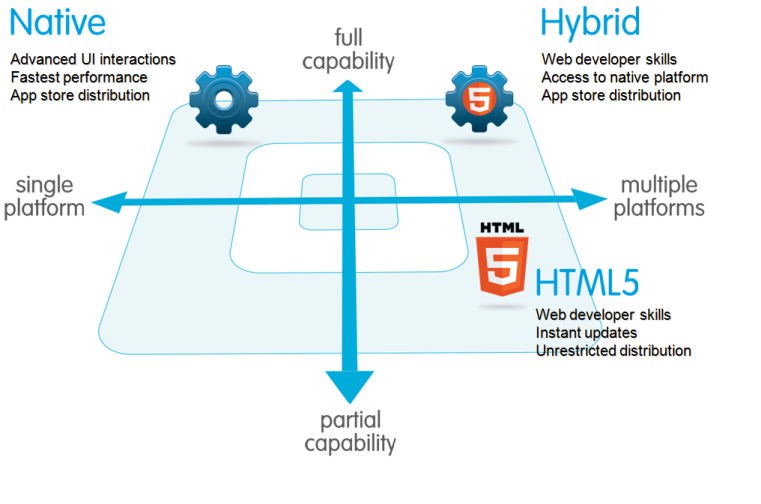
\includegraphics[width=0.9\textwidth]{../images/compare_hybrid_app.png}
  \caption[App híbrida]{App móvil híbrida (\href{https://developer.salesforce.com}{https://developer.salesforce.com}).}
  \label{fig:compare_hybrid_app}
  \end{center}
\end{figure}

Las principales ventajas de estas aplicaciones son:

\begin{itemize}
  \item \itembf{Bajo coste de desarrollo.}
  \item \itembf{Multiplataforma.}
  \item \itembf{Tiempo de desarrollo corto.}
  \item \itembf{Fácil distribución.}
\end{itemize}


\bigskip
Y lo que más nos interesa para este proyecto, sus desventajas:

\begin{itemize}
  \item \itembf{Rendimiento pobre.}
  \item \itembf{Escalabilidad baja.}
  \item \itembf{Diseño sujeto al diseño web.}
  \item \itembf{Acceso a las características especiales del hardware limitado.}
\end{itemize}


\bigskip
En un principio la aplicación que se desarrolló en el período de prácticas ICARO se planteó como una aplicación sencilla donde consultar conceptos y esquemas de las asignaturas. Los datos se consultarían desde una hoja de Google Drive común al departamento y se mostrarían en la aplicación directamente y por estas características, se .

A medida que avanzaba el desarrollo  y acercándose la fase final, el ``cliente'' planteó nuevas funcionalidades, topándonos con el primer problema: \textbf{la escalabilidad} de estas aplicaciones.



\subsection{Análisis del problema}
Una vez desarrollada esta aplicación, aunque en general quedamos contentos con el resultado, acusamos los siguientes problemas:

\begin{itemize}
  \item \itembf{No disponíamos de un servidor, toda la aplicación se ejecutaba en el cliente.}
  \item \itembf{Falta de base de datos.}
  \item \itembf{No se usa la API de Google Drive}
  \item \itembf{Acceso a Google Drive en cada sección de la aplicación}
  \item \itembf{Lentitud de acceso de datos en cada sección de la aplicación}
  \item \itembf{Mala elección de framework CSS, señales de obsoleto.}
\end{itemize}

\bigskip 
Solventar estos problemas, con el fin de iniciar un proyecto mejor planificado, con miras a una mayor escalabilidad analizando los requisitos presentes y los que pudieran surgir en un futuro, es la principal motivación para este proyecto. Aprovecharemos para mejorar la experiencia de usuario, ya que la lentitud de carga entre secciones era uno de los grandes problemas que hacían tediosa la consulta del contenido de la asignatura.

\bigskip
El primer paso importante es olvidar la tecnología móvil híbrida, que originó muchos problemas en el proyecto anterior y dividirlo en dos, una parte de desarrollo web y una parte de desarrollo móvil capaces de escalar sin problema. Nuestro proyecto se centrará en la aplicación web.


\section{Estado del arte y elección de la tecnología}
Para abordar los problemas descritos y antes de realizar un análisis más profundo se hará un estudio de las tecnologías web que pueden sernos útiles en proyectos de este tipo. Teniendo claro que vamos a desarrollar el proyecto bajo una arquitectura web y hecho el repaso de los inconvenientes en las tecnologías híbridas podemos sintetizar los siguientes puntos que necesita nuestro nuevo proyecto:

\begin{itemize}
  \item \itembf{Servir el contenido con un servidor web.}
  \item \itembf{Consultar el contenido de la hoja de Google Drive del Departamento.}
  \item \itembf{Almacenar el contenido en una base de datos.}
  \item \itembf{Gestión de usuarios.}
  \item \itembf{Establecer roles para los usuarios.}
\end{itemize}

\subsection{El lenguaje de programación}

\bigskip 
Lo primero que vamos a plantearnos es el \textbf{lenguaje} a usar, y que mejor forma de abrir un abanico de posibilidades que explorar los lenguajes más usados en la comunidad de GitHub\footnote{GitHub es una plataforma de desarrollo colaborativo donde usted puede alojar proyectos propios así como contribuir en otros proyectos. GitHub usa el sistema de control de versiones Git.} desde mediados de 2016 a mediados de 2017.

\begin{figure}[!ht]
  \begin{center}
  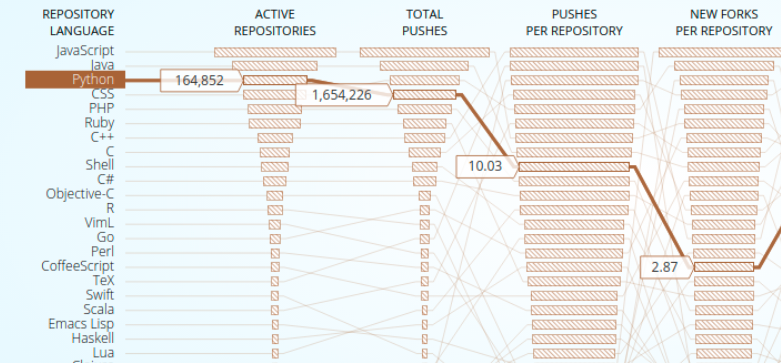
\includegraphics[width=1\textwidth]{../images/trend_lang_github_16-17.png}
  \caption[Top languages GitHub]{Top languages GitHub (\href{http://githut.info/}{http://githut.info/}).}
  \label{fig:trending_languages_github_16-17}
  \end{center}
\end{figure}

\bigskip
Como podemos ver en la figura anterior, entre los 5 lenguajes más usados se encuentran: JavaScript, Java, Python, PHP y Ruby (y sí, está CSS y lo hemos obviado ya que es un lenguaje usado únicamente para definir los estilos de un documenta HTML o XML). 

\bigskip
\textbf{JavaScript} nos ofrece la alternativa de Node.js para el lado del servidor pero no está diseñado para aplicaciones complejas. Node.js es un lenguaje interpretado y aunque trabaja de forma asíncrona, está diseñado para ejecutarse en un sólo hilo, por lo que podría presentar ciertas limitaciones a la hora de escalar en aplicaciones complejas. Además las aplicaciones con Node.js permanecen en RAM, no siendo re-interpretadas con nuevas peticiones si no que se procesa directamente desde la memoria.

\bigskip
JavaScript no se estudió profundamente durante el {\grado} y aunque descubrir e indagar en un lenguaje nuevo podría ser un aliciente, sus propiedades y las ``limitaciones'' en cuanto a la escalabilidad, que recuerdan al desarrollo en JavaScript de las aplicaciones híbridas, nos hacen descartar este lenguaje.

\bigskip
\textbf{Java} en cambio es un lenguaje que hemos profundizado más durante los años de estudio. Si es verdad que la mayoría del desarrollo que llevamos a cabo estos años era referente a aplicaciones de escritorio, pero la idea de un lenguaje nuevo o poco profundizado nos parecía más interesante en este proyecto.

\bigskip
Llegamos a los tres lenguajes que nos parecieron más interesantes para el proyecto \textbf{PHP}, \textbf{Ruby} y \textbf{Python}\cite{python_blackbook}. A una primera vista estos lenguajes eran candidatos para el desarrollo, vamos a señalar las características que se observaron para decidirnos por uno:


\bigskip
\begin{table}[htb]
\begin{tabular}{| p{4.2cm}| p{4.2cm} | p{4.2cm} |}
\hline
\multicolumn{3}{|c|}{\textbf{Características}} \\
\hline
\textbf{PHP} & \textbf{Ruby} & \textbf{Python} \\
\hline \hline \hline

Curva de aprendizaje corta & Curva de aprendizaje compleja & Curva de aprendizaje corta\\ \hline
Legibilidad y estructuración baja & Legibilidad y estructuración media & Legibilidad y estructuración alta \\ \hline
Popularidad alta & Popularidad baja & Popularidad media \\ \hline
Comunidad media & Comunidad media & Comunidad alta \\ \hline
\end{tabular}
\caption{Tabla de características.}
\label{tabla:anchofijo}
\end{table}

\bigskip
Hemos visto que PHP es el más usado en cuanto a cantidad de aplicaciones totales desarrolladas, pero a lo largo del último año, como se aprecia en la figura \ref{fig:trending_languages_github_16-17}, Python ha crecido enormemente en el número de contribuciones y en su comunidad. Viendo la evolución de este lenguaje y teniendo en cuenta sus características que ayudan a crear aplicaciones bien estructuradas, escalables, con módulos altamente reutilizables y teniendo una comunidad, tanto anglosajona como hispana, tan grande, Python será la opción elegida como lenguaje de \titulo .

\bigskip
Decir también que durante el grado se hizo una breve introducción a Python y se usó para pequeñas y aisladas aplicaciones, sintiendo una gran inquietud por usar este lenguaje en un proyecto más completo.




\subsection{Framework web}

Un framework web\cite{python_wiki, django_basic} es una colección de paquetes o módulos que permiten a los desarrolladores escribir aplicaciones o servicios web sin tener que manejar detalles de bajo nivel como protocolos, sockets o gestión de procesos.

\bigskip
Las aplicaciones web comúnmente utilizan y hacen uso de una serie de componentes, ya sea durante su desarrollo o en la etapa de producción, tales como un servidor HTTP, mecanismos de almacenamiento como podría ser una base de datos, un motor de plantillas, un conjunto de herramientas AJAX, etc. Estos framework agrupan y gestionan paquetes con estos componentes que ayudan en la abstracción del desarrollo de bajo nivel.

\bigskip
Ya que tenemos claro el lenguaje, vamos a hacer un breve estudio de los frameworks web existentes que nos permitirán un desarrollo ágil y mejor estructurado. Los tres frameworks web más importantes de Python por su volumen de proyectos, comunidad y completitud son:


\begin{itemize}
  \item {Django}
  \item {TurboGears2}
  \item {Web2Py}
\end{itemize}


\bigskip
Entre ellos, \textbf{Django}\cite{django_basic} es claramente el más usado y con una comunidad más grande. Se basa en el principio DRY\footnote{Don't Repeat Yourself} lo que propicia un desarrollo más rápido, con menos código y por consecuencia más limpio y pragmático. Django se centra en automatizar tanto como sea posible. En la documentación de Django se habla de que el framework usa un enfoque MVC\footnote{Modelo Vista Controlador}  y en la misma documentación también se habla de un enfoque MVT\footnote{Modelo Vista Template}. Esto es porque ambos enfoques están estrechamente relacionados, se habla de un MVT donde el controlador lo gestiona el propio framework trabajando el desarrollador directamente con los ``Templates''.

\bigskip
\textbf{TurboGears2}\cite{turbogears} aparece con la idea de resolver las frustraciones de otros frameworks y con la filosofía de adoptar lo mejor de otros frameworks de características similares y resolver sus puntos flacos. Framework que destaca por la agilidad en el desarrollo de aplicaciones y servicios simples y la capacidad de escalar hasta aplicaciones completas. Utiliza un concepto de modularización que permite adaptar distintos motores de plantillas y webservers. Utiliza como controlador SQLAlchemy\footnote{Conjunto de herramientas Python SQL y ORM que ofrede al desarrollador toda la flexibilidad y funcionalidad de SQL}, ORM muy bien considerado y afamado.

\bigskip
Por otro lado \textbf{Web2Py} es el más sencillo de los tres. No tiene archivos de configuración, no requiere instalación e incluso se puede ejecutar desde una unidad USB. Extendido y con una comunidad amplia está muy indicado para proyectos sencillos. Al igual que TurboGears2 utiliza la filosofía de agrupar lo mejor de otros frameworks. Utiliza la idea de MVC de Ruby On Rails  y la filosofía de forms de Django por lo que para muchos desarrolladores será muy cómodo si conocen estos frameworks.


\bigskip
Para este proyecto el framework que hemos decidido utilizar es \textbf{Django}. Al ver su comunidad, volumen de proyectos y calidad de los mismos tales como Instagram, Mozilla o Pinterest \cite{djangoproject} creemos que es el indicado para desarrollar la aplicación. Django es compatible con Python 2 y 3 y muy recomendable para proyectos con miras a una gran escalabilidad. Personalmente y antes de desarrollar {\titulo} me parece interesante ya no sólo la gran comunidad de desarrolladores también la calidad de su documentación en cuanto a explicaciones y ejemplos. Creemos por esto que es la mejor apuesta para el TFG.



\subsection{Sistema para el control de versiones}

El control de versiones se dedica a la gestión de los cambios que se realizan sobre los ficheros o configuraciones. Una revisión o versión de un fichero es el estado en el que se encuentra este en cierto momento de su desarrollo.

\bigskip
Un sistema de control de versiones facilita la administración de las distintas versiones del código o el producto desarrollado, así como las posibles especializaciones realizadas, ya sea para una bifurcación del desarrollo en un punto del proyecto o para mantener una versión estable en producción mientras se desarrolla un proyecto.

\bigskip
Durante el {\grado} hemos trabajado con Git como sistema de control de versiones satisfaciendo totalmente las necesidades de los desarrollos. No encontramos razones para dejar Git y utilizar otros sistemas.Aún así se indagó en otras opciones comunes en el desarrollo de proyectos encontrando dos opciones en la mayoría de estos: Git y SubVersion. Las principales características son:

\begin{itemize}
\item [\textbf{Git}]
\item Control de versiones distribuido.
\item Se trabaja sobre copias locales del repositorio.
\item Autorización para la totalidad del repositorio.
\item Sólo es necesaria conexión para la sincronización.
\item [\textbf{SubVersion}]
\item Control de versiones centralizado.
\item Repositorio central donde se generan copias de trabajo.
\item Autorización sobre rutas concretas del repositorio.
\item Necesaria conexión a la red con cada acceso.
\end{itemize}


Ya que necesitamos un repositorio donde poder trabajar con o sin conexión a internet, excepto cuando necesitemos sincronizar nuestro trabajo local, y no necesitamos un control de permisos sobre rutas específicas del repositorio, tendremos acceso al repositorio completo, seguimos pensando que Git es la mejor opción.

\bigskip
Aunque hablaremos de ello más adelante, vamos a tener la precaución de dividir los repositorios del proyecto en dos. Un repositorio será destinado al código fuente y otro a la documentación. Esto nos ayudará en el momento de desplegar la aplicación en un servidor de desarrollo ya que podremos subir los ficheros fuente independientemente sin tener que manejar los ficheros de la documentación en el mismo repositorio.



\subsection{Entorno de desarrollo}

En un primer momento se pensó en desarrollar la aplicación sin ningún entorno de desarrollo integrado (IDE), simplemente bajo un editor de texto y las herramientas de terminal necesarias. Se planteó esta idea por dos razones principales. La primera que se buscaban herramientas livianas que no aumentaran mucho la carga de procesamiento del equipo en el que se iba a desarrollar y la segunda es que durante el grado nos hemos topado con problemas de los entornos de desarrollo al automatizar muchas tareas, si bien es cierto que esto abstrae al desarrollador de procedimientos repetitivos (por ejemplo lanzar el servidor desde la terminal cada vez que se realizan ciertos cambios en el desarrollo) también puede ser contraproducente al no controlar de forma manual todas estas tareas. Aún así esto siempre dependerá del desarrollador y del buen o mal uso que haga de estos entornos de desarrollo.

\bigskip
Como decimos, las primeras pruebas se desarrollaron en un editor de textos y una terminal, comprendiendo la instalación de Python y Django, sus paquetes, el entorno virtual, etc. Pronto nos topamos con algunas dificultades a la hora de desarrollar las primeras funcionalidades dentro del entorno virtual de prueba y es que al ser tecnologías nuevas para nosotros, con una sintaxis nueva y una metodología de Django un poco peculiar, invertíamos mucho tiempo en ver si lo que programado estaba bien o no, si había errores de sintaxis, o si la forma era la correcta. Por esto decidimos investigar un poco en los IDE y probar alguno antes de dejar los entornos de prueba y empezar el desarrollo.

\bigskip
Durante el grado si hemos usado un IDE en algunas asignaturas este ha sido NetBeans y es el primero que exploramos pero, desgraciadamente, no es la mejor opción para Django. Si bien es cierto que encontramos artículos sobre cómo crear proyectos Django con NetBeans, también encontramos muchos artículos desaconsejándolo ya que aunque existen paquetes para poder trabajar con Django, no son muy estables, y al intentar crear un nuevo proyecto de prueba hemos encontrado problemas como :

\begin{itemize}
  \item Variables de entorno no localizables.
  \item NetBeans funciona mal con el entorno virtual.
  \item Paquetes para Django antiguos y desactualizados.
\end{itemize}

Por esto y sin dedicar mucho a intentar solucionar con paquetes externos estos problemas pasamos al siguiente IDE ya recomendado por compañeros del Grado para Django: PyCharm. Este IDE a diferencia de NetBeans está totalmente integrado con Python y Django y las características que más agilidad van a aportar al desarrollo son:

\begin{itemize}
  \item Entorno virtual totalmente integrado. Al arrancar el proyecto ya dispones de una consola en este.
  \item Consola Python con la versión actualmente utilizada.
  \item Arranca el servidor con el atajo de teclado Mayus+F10.
  \item Sincronización con el control de versiones utilizado en el entorno virtual.
\end{itemize}

\bigskip
En las figuras \ref{fig:pycharm1} y \ref{fig:pycharm2} podemos ver dos capturas de pantalla del entorno de desarrollo.

\begin{figure}[!h]
  \begin{center}
  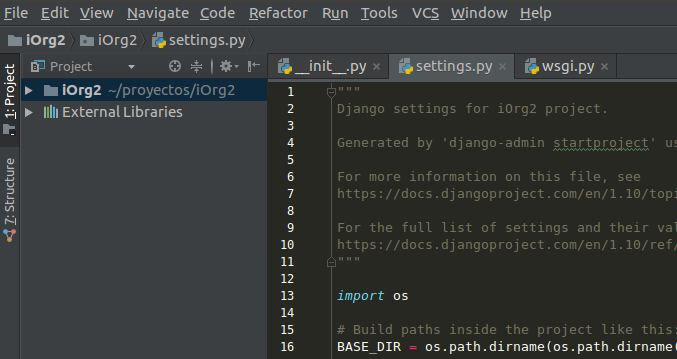
\includegraphics[width=0.6\textwidth]{../images/pycharm1.png}
  \caption[Pycharm 1/2]{ Captura de pantalla de la zona del proyecto }
  \label{fig:pycharm1}
  \end{center}
\end{figure}

\begin{figure}[!h]
  \begin{center}
  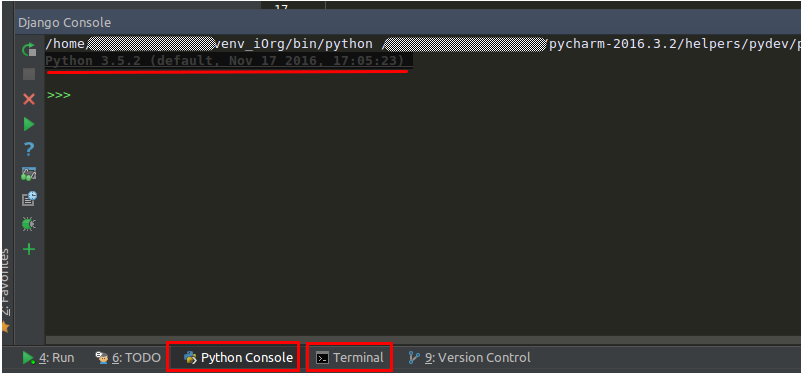
\includegraphics[width=0.6\textwidth]{../images/pycharm2.png}
  \caption[Pycharm 2/2]{ Captura de pantalla de la zona de la consola }
  \label{fig:pycharm2}
  \end{center}
\end{figure}

\bigskip
Además JetBrains\footnote{JetBrains: compañía desarrolladora de PyCharm (\href{https://www.jetbrains.com/}{https://www.jetbrains.com/})} ofrece el paquete profesional de PyCharm gratuito a estudiantes al que podemos acceder registrando nuestro correo de estudiante de la Universidad de Granada.

\bigskip 
Por las pruebas realizadas y las ventajas que ofrece vamos a utilizar PyCharm como IDE.




\chapter{Objetivos}\label{sec:objetives}

{\titulo} persigue el objetivo general de desarrollar una aplicación web de apoyo a la docencia para las asignaturas del Departamento de Organización de Empresas de la Facultad de Ciencias Económicas y Empresariales de la Universidad de Granada. Esta aplicación deberá obtener los datos de una hoja de cálculo de Google Drive en la cual los profesores de dicho departamento tienen información docente de sus asignaturas, y trabajar con estos datos para mostrarlos al alumno. Seguiremos la filosofía de \textbf{Software Libre} heredada del anterior proyecto.


\bigskip
A continuación vamos a listar los objetivos principales:

\begin{itemize}
  \item \textbf{OBJ-P-1.} Conseguir una primera versión funcional de la aplicación donde un alumno pueda consultar los conceptos y resolver algunas preguntas de la asignatura.
  \item \textbf{OBJ-P-2.} El proyecto debe estar estructurado de forma que sea escalable, permitiendo añadir en un futuro nuevas funcionalidades no dependientes de las actuales.
  \item \textbf{OBJ-P-3.} Conexión segura con Google Drive mediante su API.
  \item \textbf{OBJ-P-4.} Solventar los problemas de latencia al navegar entre secciones de la versión anterior.
  \item \textbf{OBJ-P-5.} Heredar el principio de Software Libre de la versión anterior, publicando este proyecto en GitHub y permitiendo a la comunidad participar en él.
\end{itemize}


\bigskip
También propondremos unos objetivos secundarios, que se intentarán alcanzar en la medida de lo posible:

\begin{itemize}
  \item \textbf{OBJ-S-1.} Añadir estadísticas básicas sobre la actividad de los alumnos en la aplicación.

  \item \textbf{OBJ-S-2.} Adaptar las vistas de la aplicación web a los tamaños de resolución de diferentes dispositivos.
  
  \item \textbf{OBJ-S-3.} Tener en cuenta el uso de la aplicación desde entornos con internet de velocidad limitada, mejorando así su usabilidad.

  \item \textbf{OBJ-S-4.} Despliegue de la aplicación en PaaS\footnote{``Platform as a Service''. Plataforma y entorno que permite a los desarrolladores crear y ejecutar aplicaciones totalmente en la nube}.
  \item \textbf{OBJ-S-5.} Gestión de los usuarios y sus roles, al menos permisos de alumnos y profesores.
  \item \textbf{OBJ-S-6.} Consulta, por parte de los profesores, de las estadísticas generadas por los alumnos, siendo estas útiles para valorar la actividad de los alumnos en la aplicación.
\end{itemize}



\bigskip
Para el desarrollo de este proyecto vamos a hacer uso de los conocimientos adquiridos en las siguientes asignaturas del {\grado}:

\begin{itemize}
  \item \textbf{Fundamentos de programación}, base  para cualquier desarrollo.
  \item \textbf{Programación orientada a objetos}, para entender este paradigma de programación.
  \item \textbf{Ingeniería del software}, para hacer un correcto análisis y planificación de un proyecto.
  \item \textbf{Base de datos}, para comprender la gestión de las bases de datos necesarias en este proyecto. 
  \item \textbf{Diseño de Aplicaciones para Internet}, donde vimos una breve introducción a Python, Django y el uso de varias APIs de Google. 
  \item \textbf{Infraestructura virtual}, para comprender el uso de sistemas PaaS, entornos virtuales, despliegue de aplicaciones y Git como sistema de control de versiones.
\end{itemize}


\section{Repercusión de los objetivos}
El desarrollo de este proyecto debería resolver los objetivos principales para crear una base de proyecto en el cual se podrá seguir trabajando en un futuro y crear un apoyo docente para las asignaturas de el Departamento de Organización de Empresas. Con estos objetivos se crea una base de un desarrollo escalable, en el que se podrán incluir sin problemas nuevas funcionalidades completando cada vez más este proyecto.

\bigskip
Los objetivos secundarios darán más consistencia al proyecto mejorando su rendimiento, expansión y usabilidad, así como un valor añadido para las asignaturas del departamento, facilitando la labor de docentes y el aprendizaje de los alumnos. Se podrá también tener un primer acercamiento por parte de la comunidad docente al desplegarla en un PaaS y estudiar las carencias y virtudes tras su uso.


%\section{Conexión entre los objetivos}

%\input{chapters/04_Planificacion}
%\chapter{Análisis}

Siguiendo las necesidades del cliente sintetizadas en los objetivos[\ref{sec:objetives}] iniciaremos el análisis de los requisitos de la aplicación. Dividiremos la fase de análisis en dos: análisis de los requisitos funcionales y no funcionales \cite{ing_software}.

\section{Análisis de los requisitos funcionales}

Los requisitos funcionales son las características requeridas del sistema que expresan una funcionalidad de este:


\begin{itemize}
	\item \textbf{RF-1.} Consulta de datos de una hoja de cálculo de Google Drive
	\item \textbf{RF-2.} Mostrar conceptos de la asignatura
	\item \textbf{RF-3.} Se deberá generar preguntas aleatorias de cada tema. Las preguntas deberán estar diferenciadas en dos tipos:
		\begin{itemize}
			\item \textbf{RF-3.1.} Generación de pregunta tipo test con varias opciones y sólo una seleccionable.
			\item \textbf{RF-3.2.} Generación de pregunta verdadero/falso.
		\end{itemize}
	\item \textbf{RF-4.} Se deberá generar un examen de 20 preguntas aleatorias del tipo de preguntas seleccionado.
	\item \textbf{RF-5.} Se generarán estadísticas básicas de las actividades realizadas por cada alumno en la aplicación. 
		\begin{itemize}
			\item \textbf{RF-5.1.} Número de preguntas correctas e incorrectas.
			\item \textbf{RF-5.2.} Número de exámenes aprobados y suspendidos.
			\item \textbf{RF-5.3.} Nota media de los exámenes aprobados y suspendidos así como la nota media total.
		\end{itemize}
	\item \textbf{RF-6.} Los profesores podrán consultar las estadísticas de los alumnos.
	\item \textbf{RF-7.} Los profesores podrán actualizar los datos de la aplicación, estos se leerán de la hoja de cálculo de Google Drive.
	\item \textbf{RF-8.} Gestión de los usuarios de la aplicación.
\end{itemize}


\section{Análisis de los requisitos no funcionales}

Los requisitos no funcionales hacen referencia a las cualidades del producto requeridas por el cliente. Estas características no se limitan a la aplicación, pueden ser referentes al sistema, al proceso de desarrollo o incluso al entorno.

\begin{itemize}
  \item \textbf{RNF-1.} Rendimiento. Especial cuidado con la velocidad de carga entre secciones.
  \item \textbf{RNF-2.} Conceptos y preguntas se agruparán por temas.
  \item \textbf{RNF-3.}\label{rnf-3} La aplicación se visualizará desde diversos dispositivos, atender a las diferentes resoluciones de pantalla.
  \item \textbf{RNF-4.} Eficiencia en el uso y descarga de datos. Esto es, por ejemplo, el usuario que consulta la aplicación no deberá descargar todo el contenido de la hoja, sólo deberá descargar los datos de la sección consultada.
\end{itemize}


\section{Casos de uso}
	Los casos de uso son una técnica para especificar el comportamiento de un sistema. Hacen referencia a los procedimientos llevados a cabo entre el sistema y una entidad para dar una funcionalidad. Las entidades que participan en estas interacciones con el sistema se denominan actores.

\subsection{Actores}

	
\begin{itemize}
  \item \textbf{Ac-1. Usuario anónimo.}
  \begin{itemize}
   \item \textbf{Descripción:} Persona que visita la aplicación.
   \item \textbf{Características:} Es el usuario que llega por primera vez a la aplicación.
   \item \textbf{Relaciones:} Ninguna.
   \item \textbf{Atributos:} Ninguno.
   \item \textbf{Comentarios:} Este usuario no puede hacer uso de la aplicación más que ver que actividades se desarrollan o alguna información sobre el proyecto.
  \end{itemize}
\end{itemize}

\begin{itemize}
  \item \textbf{Ac-2. Usuario alumno.}
  \begin{itemize}
   \item \textbf{Descripción:} Persona que ha iniciado sesión en la aplicación.
   \item \textbf{Características:} Es el usuario que puede realizar las actividades docentes de la asignatura.
   \item \textbf{Relaciones:} Ninguna.
   \item \textbf{Atributos:} usuario, contraseña, nombre, apellidos y email.
   \item \textbf{Comentarios:} No tiene permisos de administración.
  \end{itemize}
\end{itemize}

\begin{itemize}
  \item \textbf{Ac-3. Usuario profesor.}
  \begin{itemize}
   \item \textbf{Descripción:} Persona que visita la aplicación.
   \item \textbf{Características:} Usuario con permisos de administración de la información docente.
   \item \textbf{Relaciones:} Ninguna.
   \item \textbf{Atributos:} usuario, contraseña, nombre, apellidos y email.
   \item \textbf{Comentarios:} Podrá consultar las estadísticas generadas de los usuarios alumnos.
  \end{itemize}
\end{itemize}

\begin{itemize}
  \item \textbf{Ac-4. Usuario administrador.}
  \begin{itemize}
   \item \textbf{Descripción:} Es el administrador del sistema.
   \item \textbf{Características:} Usuario que puede gestionar los demás usuarios, así como dar permisos al usuario profesor.
   \item \textbf{Relaciones:} Ninguna.
   \item \textbf{Atributos:} usuario, contraseña y email.
   \item \textbf{Comentarios:} Aunque no se restrinja, este usuario no está destinado al uso de la aplicación más allá de las labores de gestión del sistema.
  \end{itemize}
\end{itemize}


\subsection{Casos de uso}

\begin{itemize}
  \item \textbf{CU-1.} Inicio de sesión en el sistema.
  \begin{itemize}
    \item \textbf{Actores:} Usuario anónimo.
    \item \textbf{Tipo:} Primario, esencial.
    \item \textbf{Referencias:}
    \item \textbf{Precondición:} No tener iniciada una sesión previamente.
    \item \textbf{Postcondición:} El usuario anónimo pasará a ser ususario alumno ó ususario profesor.
    \item \textbf{Autor:} \autor.
    \item \textbf{Versión:} 1.0.
    \item \textbf{Propósito:} Pasar a ser un usuario con la sesión iniciada en el sistema.
    \item \textbf{Resumen:} El usuario introducirá su nombre de usuario y su contraseña para iniciar sesión.

    \end{itemize}
    \begin{table}[!ht]
      \begin{center}
	\begin{tabular}{|l|l|l|l|}
	  \hline
	  \multicolumn{4}{|c|}{{\bf Curso normal}}
	  \\ \hline
	  \multicolumn{2}{|c|}{{\bf Actor}} & \multicolumn{2}{c|}{{\bf Sistema}}
	  \\ \hline
	  {\it 1} & 
	  \begin{tabular}[c]{@{}l@{}}
	    El usuario hace click en el\\
	    botón ``Iniciar sesión''. \\
	  \end{tabular} &
	  &
	  \\ \hline
	  &
	  &
	  {\it 2} &
	  \begin{tabular}[c]{@{}l@{}}
	    El sistema muestra el formulario\\
	    para inicio de sesión. \\
	  \end{tabular}
	  \\ \hline
	  {\it 3} & 
	  \begin{tabular}[c]{@{}l@{}}
	    El usuario rellena los campos del \\
	    formulario y pulsa el botón ``Iniciar sesión''. \\
	  \end{tabular} &
	  &
	  \\ \hline
	  &
	  &
	  {\it 4a} &
	  \begin{tabular}[c]{@{}l@{}}
	    El sistema valida el usuario y\\
	    la contraseña y si ambos están\\
	    bien y coinciden inicia la \\
	    sesión de ususario. \\
	  \end{tabular}
	  \\ \hline
	\end{tabular}
	\caption{CU-1. Inicio de sesión.}
	\label{table:cu_1}
      \end{center}
    \end{table}
    
    \begin{table}[!ht]
      \begin{center}
	\begin{tabular}{|l|l|}
	  \hline
	  \multicolumn{2}{|c|}{{\bf Curso alterno}}
	  \\ \hline
	  {\it 4b} &
	  \begin{tabular}[c]{@{}l@{}}
	    Si algo ha ido mal en la validación  del usuario y contraseña, \\
	    el sistema vuelve al paso 2 de CU-1 (tabla \ref{table:cu_1}).
	  \end{tabular}\\
	  \hline
	\end{tabular}
	\caption{Curso alterno de CU-1. Inicio de sesión.}
	\label{table:cu_1_ca}
      \end{center}
    \end{table}

    \newpage






  \item \textbf{CU-2.} Registro en el sistema.
  \begin{itemize}
    \item \textbf{Actores:} Usuario alumno.
    \item \textbf{Tipo:} Primario, esencial.
    \item \textbf{Referencias:}
    \item \textbf{Precondición:} No tener iniciada una sesión previamente.
    \item \textbf{Postcondición:} El usuario tendrá una cuenta con la que iniciar sesión.
    \item \textbf{Autor:} \autor.
    \item \textbf{Versión:} 1.0.
    \item \textbf{Propósito:} Tener una cuenta de usuario alumno.
    \item \textbf{Resumen:} El usuario rellenará un formulario de registro del sistema y si todo va bien, tendrá una cuenta con la que iniciar sesión.

    \end{itemize}
    \begin{table}[!ht]
      \begin{center}
	\begin{tabular}{|l|l|l|l|}
	  \hline
	  \multicolumn{4}{|c|}{{\bf Curso normal}}
	  \\ \hline
	  \multicolumn{2}{|c|}{{\bf Actor}} & \multicolumn{2}{c|}{{\bf Sistema}}
	  \\ \hline
	  {\it 1} & 
	  \begin{tabular}[c]{@{}l@{}}
	    El usuario hace click en el botón\\
	    ``Registrarse''. \\
	  \end{tabular} &
	  &
	  \\ \hline
	  &
	  &
	  {\it 2} &
	  \begin{tabular}[c]{@{}l@{}}
	    El sistema muestra el formulario\\
	    para registrar un usuario. \\
	    En este formulario se pedirán: \\
	    nombre de usuario, contraseña, e-mail, \\
	    nombre y apellidos.
	  \end{tabular}
	  \\ \hline
	  {\it 3} & 
	  \begin{tabular}[c]{@{}l@{}}
	    El ususario rellena el formulario \\
	    y lo envía con el botón ``Registrar''. \\
	  \end{tabular} &
	  &
	  \\ \hline
	  &
	  &
	  {\it 4a} &
	  \begin{tabular}[c]{@{}l@{}}
	    El sistema valida los datos \\
	    y sin son correctos el sistema \\
	    registra el usuario.\\
	  \end{tabular}
	  \\ \hline
	\end{tabular}
	\caption{CU-1. Inicio de sesión.}
	\label{table:cu_2}
      \end{center}
    \end{table}
    
    \begin{table}[!ht]
      \begin{center}
	\begin{tabular}{|l|l|}
	  \hline
	  \multicolumn{2}{|c|}{{\bf Curso alterno}}
	  \\ \hline
	  {\it 4b} &
	  \begin{tabular}[c]{@{}l@{}}
	    Si algo ha ido mal en la validación  del formulario, \\
	    el sistema vuelve al paso 2 de CU-2 (tabla \ref{table:cu_2}).
	  \end{tabular}\\
	  \hline
	\end{tabular}
	\caption{Curso alterno de CU-2. Registro en el sistema.}
	\label{table:cu_2_ca}
      \end{center}
    \end{table}


\newpage






  \item \textbf{CU-3.} Cerrar sesión.
  \begin{itemize}
    \item \textbf{Actores:} Usuario alumno, usuario profesor, usuario administrador.
    \item \textbf{Tipo:} Primario.
    \item \textbf{Referencias:}
    \item \textbf{Precondición:} Tener una sesión iniciada.
    \item \textbf{Postcondición:} El usuario no tendrá la sesión iniciada.
    \item \textbf{Autor:} \autor.
    \item \textbf{Versión:} 1.0.
    \item \textbf{Propósito:} Cerrar la sesión de un usuario en el sistema.
    \item \textbf{Resumen:} El usuario pulsará el botón de cerrar sesión y el sistema cerrará la misma, volviendo a la pantalla de inicio de sesión paso 2 de CU-1 (tabla \ref{table:cu_1}).

    \end{itemize}
    \begin{table}[!ht]
      \begin{center}
	\begin{tabular}{|l|l|l|l|}
	  \hline
	  \multicolumn{4}{|c|}{{\bf Curso normal}}
	  \\ \hline
	  \multicolumn{2}{|c|}{{\bf Actor}} & \multicolumn{2}{c|}{{\bf Sistema}}
	  \\ \hline
	  {\it 1} & 
	  \begin{tabular}[c]{@{}l@{}}
	    El usuario hace click en el botón\\
	    ``Cerrar sesión''. \\
	  \end{tabular} &
	  &
	  \\ \hline
	  &
	  &
	  {\it 2} &
	  \begin{tabular}[c]{@{}l@{}}
	    El sistema cierra la sesión del usuario\\
	    y vuelve al paso 2 de CU-1 (tabla \ref{table:cu_1})
	  \end{tabular}
	  \\ \hline
	\end{tabular}
	\caption{CU-3. Cerrar sesión.}
	\label{table:cu_3}
      \end{center}
    \end{table}





\newpage






  \item \textbf{CU-4.} Consulta estadísticas propias.
  \begin{itemize}
    \item \textbf{Actores:} Usuario alumno, usuario profesor.
    \item \textbf{Tipo:} Primario, esencial.
    \item \textbf{Referencias:}
    \item \textbf{Precondición:} Tener iniciada una sesión de usuario.
    \item \textbf{Postcondición:} - 
    \item \textbf{Autor:} \autor.
    \item \textbf{Versión:} 1.0.
    \item \textbf{Propósito:} El usuario consulta sus estadísticas.
    \item \textbf{Resumen:} El usuario consultará sus estadísticas creadas a partir del uso de la aplicación.

    \end{itemize}
    \begin{table}[!ht]
      \begin{center}
	\begin{tabular}{|l|l|l|l|}
	  \hline
	  \multicolumn{4}{|c|}{{\bf Curso normal}}
	  \\ \hline
	  \multicolumn{2}{|c|}{{\bf Actor}} & \multicolumn{2}{c|}{{\bf Sistema}}
	  \\ \hline
	  {\it 1} & 
	  \begin{tabular}[c]{@{}l@{}}
	    El usuario hace click en el botón\\
	    ``Perfil''. \\
	  \end{tabular} &
	  &
	  \\ \hline
	  &
	  &
	  {\it 2} &
	  \begin{tabular}[c]{@{}l@{}}
	    El sistema muestra el perfil del \\
	    usuario con su nombre de usuario \\
	    y sus estadísticas básicas: número de\\
	    preguntas correctas e incorrectas,\\
	    número de exámenes aprobados y suspensos,\\
	    nota media de exámenes aprobados y suspensos\\
	    y la nota media total de los exámenes realizados.
	  \end{tabular}
	  \\ \hline
	\end{tabular}
	\caption{CU-4. Consulta estadísticas propias.}
	\label{table:cu_4}
      \end{center}
    \end{table}


        \newpage





  \item \textbf{CU-5.} Consultar concepto de un tema.
  \begin{itemize}
    \item \textbf{Actores:} Usuario alumno, usuario profesor.
    \item \textbf{Tipo:} Primario, esencial.
    \item \textbf{Referencias:}
    \item \textbf{Precondición:} Tener una sesión iniciada.
    \item \textbf{Postcondición:} -
    \item \textbf{Autor:} \autor.
    \item \textbf{Versión:} 1.0.
    \item \textbf{Propósito:} Consultar un concepto.
    \item \textbf{Resumen:} El usuario consulta el concepto deseado de un tema concreto.

    \end{itemize}
    \begin{table}[!ht]
      \begin{center}
	\begin{tabular}{|l|l|l|l|}
	  \hline
	  \multicolumn{4}{|c|}{{\bf Curso normal}}
	  \\ \hline
	  \multicolumn{2}{|c|}{{\bf Actor}} & \multicolumn{2}{c|}{{\bf Sistema}}
	  \\ \hline
	  {\it 1} & 
	  \begin{tabular}[c]{@{}l@{}}
	    El usuario hace click en el botón\\
	    ``Conceptos''. \\
	  \end{tabular} &
	  &
	  \\ \hline
	  &
	  &
	  {\it 2} &
	  \begin{tabular}[c]{@{}l@{}}
	    El sistema muestra una lista\\
	    con los temas que  contiene a \\
	    los conceptos.
	  \end{tabular}
	  \\ \hline
	  {\it 3} & 
	  \begin{tabular}[c]{@{}l@{}}
	    El usuario pulsa sobre el tema\\
	    deseado.
	  \end{tabular} &
	  &
	  \\ \hline
	  &
	  &
	  {\it 4a} &
	  \begin{tabular}[c]{@{}l@{}}
	    El sistema muestra las secciones\\
	    en las que están agrupados los conceptos\\
	    dentro de los temas.
	  \end{tabular}
	  \\ \hline
	  {\it 5} & 
	  \begin{tabular}[c]{@{}l@{}}
	    El usuario pulsa sobre la\\
	    sección en que se encuentra el\\
	    concepto.
	  \end{tabular} &
	  &
	  \\ \hline
	  &
	  &
	  {\it 6} &
	  \begin{tabular}[c]{@{}l@{}}
	    El sistema muestra los\\
	    conceptos que contiene esa \\
	    sección del tema.
	  \end{tabular}
	  \\ \hline
	  {\it 7} & 
	  \begin{tabular}[c]{@{}l@{}}
	    El usuario pulsa sobre el concepto\\
	    deseado.
	  \end{tabular} &
	  &
	  \\ \hline
	  &
	  &
	  {\it 8} &
	  \begin{tabular}[c]{@{}l@{}}
	    El sistema muestra una\\
	    pantalla con la información\\
	    de ese concepto: nombre, definición\\
	    ejemplo y figura(opcional).
	  \end{tabular}
	  \\ \hline
	\end{tabular}
	\caption{CU-5. Consultar concepto.}
	\label{table:cu_5}
      \end{center}
    \end{table}
    
    \begin{table}[!ht]
      \begin{center}
	\begin{tabular}{|l|l|}
	  \hline
	  \multicolumn{2}{|c|}{{\bf Curso alterno}}
	  \\ \hline
	  {\it 4b} &
	  \begin{tabular}[c]{@{}l@{}}
	    Si el tema no tiene secciones el sitema nos \\
	    llevará al paso 6 de CU-5 (tabla \ref{table:cu_5}).
	  \end{tabular}\\
	  \hline
	\end{tabular}
	\caption{Curso alterno de CU-5. Consultar concepto de un tema.}
	\label{table:cu_5_ca}
      \end{center}
    \end{table}



        \newpage



        \newpage




  \item \textbf{CU-6.} Resolver pregunta tipo test con varias opciones y una sola respuesta.
  \begin{itemize}
    \item \textbf{Actores:} Usuario alumno, usuario profesor.
    \item \textbf{Tipo:} Primario, esencial.
    \item \textbf{Referencias:}
    \item \textbf{Precondición:} Tener una sesión iniciada.
    \item \textbf{Postcondición:} -
    \item \textbf{Autor:} \autor.
    \item \textbf{Versión:} 1.0.
    \item \textbf{Propósito:} Resolver una pregunta tipo test.
    \item \textbf{Resumen:} El usuario entra en la sección preguntas y resuelve una pregunta aleatoria del tipo y tema seleccionados.

    \end{itemize}
    \begin{table}[!ht]
      \begin{center}
	\begin{tabular}{|l|l|l|l|}
	  \hline
	  \multicolumn{4}{|c|}{{\bf Curso normal}}
	  \\ \hline
	  \multicolumn{2}{|c|}{{\bf Actor}} & \multicolumn{2}{c|}{{\bf Sistema}}
	  \\ \hline
	  {\it 1} & 
	  \begin{tabular}[c]{@{}l@{}}
	    El usuario hace click en el botón\\
	    ``Autoevaluación''. \\
	  \end{tabular} &
	  &
	  \\ \hline
	  &
	  &
	  {\it 2} &
	  \begin{tabular}[c]{@{}l@{}}
	    El sistema muestra una lista\\
	    los tipos de preguntas disponibles.
	  \end{tabular}
	  \\ \hline
	  {\it 3} & 
	  \begin{tabular}[c]{@{}l@{}}
	    El usuario pulsa sobre el tipo\\
	    ``Preguntas opción múltiple'''.
	  \end{tabular} &
	  &
	  \\ \hline
	  &
	  &
	  {\it 4} &
	  \begin{tabular}[c]{@{}l@{}}
	    El sistema muestra una lista\\
	    de temas en los que están\\
	    agrupadas las preguntas.
	  \end{tabular}
	  \\ \hline
	  {\it 5} & 
	  \begin{tabular}[c]{@{}l@{}}
	    El usuario pulsa sobre el\\
	    tema del que quiere resolver\\
	    la pregunta.
	  \end{tabular} &
	  &
	  \\ \hline
	  &
	  &
	  {\it 6} &
	  \begin{tabular}[c]{@{}l@{}}
	    El sistema buscar\\
	    aleatoriamente una pregunta\\
	    de este tema y la muestra\\
	    al usuario con un enunciado\\
	    y una lista de opciones.
	  \end{tabular}
	  \\ \hline
	  {\it 7} & 
	  \begin{tabular}[c]{@{}l@{}}
	    El usuario elige una de las\\
	    opciones como solución a la\\
	    pregunta y pulsa ``Corregir'''.
	  \end{tabular} &
	  &
	  \\ \hline
	  &
	  &
	  {\it 8} &
	  \begin{tabular}[c]{@{}l@{}}
	    El sistema muestra una\\
	    pantalla con la correción\\
	    de la pregunta mostrando \\
	    el enunciado, si es correcta\\
	    o no y una breve explicación.
	  \end{tabular}
	  \\ \hline
	\end{tabular}
	\caption{CU-6. Resolver pregunta de varias opciones y una respuesta.}
	\label{table:cu_6}
      \end{center}
    \end{table}
    



  \newpage


  \item \textbf{CU-7.} Resolver pregunta tipo test verdadero/falso.
  \begin{itemize}
    \item \textbf{Actores:} Usuario alumno, usuario profesor.
    \item \textbf{Tipo:} Primario, esencial.
    \item \textbf{Referencias:}
    \item \textbf{Precondición:} Tener una sesión iniciada.
    \item \textbf{Postcondición:} -
    \item \textbf{Autor:} \autor.
    \item \textbf{Versión:} 1.0.
    \item \textbf{Propósito:} Resolver una pregunta tipo test verdadero/falso.
    \item \textbf{Resumen:} El usuario entra en la sección preguntas y resuelve una pregunta aleatoria del tipo verdadero/falso y tema del seleccionado.

    \end{itemize}
    \begin{table}[!ht]
      \begin{center}
	\begin{tabular}{|l|l|l|l|}
	  \hline
	  \multicolumn{4}{|c|}{{\bf Curso normal}}
	  \\ \hline
	  \multicolumn{2}{|c|}{{\bf Actor}} & \multicolumn{2}{c|}{{\bf Sistema}}
	  \\ \hline
	  {\it 1} & 
	  \begin{tabular}[c]{@{}l@{}}
	    El usuario hace click en el botón\\
	    ``Autoevaluación''. \\
	  \end{tabular} &
	  &
	  \\ \hline
	  &
	  &
	  {\it 2} &
	  \begin{tabular}[c]{@{}l@{}}
	    El sistema muestra una lista\\
	    los tipos de preguntas disponibles.
	  \end{tabular}
	  \\ \hline
	  {\it 3} & 
	  \begin{tabular}[c]{@{}l@{}}
	    El usuario pulsa sobre el tipo\\
	    ``Preguntas verdadero/falso'''.
	  \end{tabular} &
	  &
	  \\ \hline
	  &
	  &
	  {\it 4} &
	  \begin{tabular}[c]{@{}l@{}}
	    El sistema muestra una lista\\
	    de temas en los que están\\
	    agrupadas las preguntas.
	  \end{tabular}
	  \\ \hline
	  {\it 5} & 
	  \begin{tabular}[c]{@{}l@{}}
	    El usuario pulsa sobre el\\
	    tema del que quiere resolver\\
	    la pregunta.
	  \end{tabular} &
	  &
	  \\ \hline
	  &
	  &
	  {\it 6} &
	  \begin{tabular}[c]{@{}l@{}}
	    El sistema buscar\\
	    aleatoriamente una pregunta\\
	    de este tema y la muestra\\
	    al usuario con un enunciado\\
	    y las opciones verdadero/falso.
	  \end{tabular}
	  \\ \hline
	  {\it 7} & 
	  \begin{tabular}[c]{@{}l@{}}
	    El usuario elige una de las\\
	    opciones como solución a la\\
	    pregunta y pulsa ``Corregir'''.
	  \end{tabular} &
	  &
	  \\ \hline
	  &
	  &
	  {\it 8} &
	  \begin{tabular}[c]{@{}l@{}}
	    El sistema muestra una\\
	    pantalla con la correción\\
	    de la pregunta mostrando \\
	    el enunciado, si es correcta\\
	    o no y una breve explicación.
	  \end{tabular}
	  \\ \hline
	\end{tabular}
	\caption{CU-7. Resolver pregunta tipo test verdadero/falso.}
	\label{table:cu_7}
      \end{center}
    \end{table}
    




    \newpage


  \item \textbf{CU-8.} Resolver examen tipo test de preguntas con varias opciones y una respuesta.
  \begin{itemize}
    \item \textbf{Actores:} Usuario alumno, usuario profesor.
    \item \textbf{Tipo:} Primario, esencial.
    \item \textbf{Referencias:}
    \item \textbf{Precondición:} Tener una sesión iniciada.
    \item \textbf{Postcondición:} -
    \item \textbf{Autor:} \autor.
    \item \textbf{Versión:} 1.0.
    \item \textbf{Propósito:} Resolver un examen tipo test.
    \item \textbf{Resumen:} El usuario resuelve un examen de preguntas con opcion múltiple.

    \end{itemize}
    \begin{table}[!ht]
      \begin{center}
	\begin{tabular}{|l|l|l|l|}
	  \hline
	  \multicolumn{4}{|c|}{{\bf Curso normal}}
	  \\ \hline
	  \multicolumn{2}{|c|}{{\bf Actor}} & \multicolumn{2}{c|}{{\bf Sistema}}
	  \\ \hline
	  {\it 1} & 
	  \begin{tabular}[c]{@{}l@{}}
	    El usuario hace click en el botón\\
	    ``Examen''. \\
	  \end{tabular} &
	  &
	  \\ \hline
	  &
	  &
	  {\it 2} &
	  \begin{tabular}[c]{@{}l@{}}
	    El sistema muestra una lista\\
	    con los tipos de exámenes disponibles.
	  \end{tabular}
	  \\ \hline
	  {\it 3} & 
	  \begin{tabular}[c]{@{}l@{}}
	    El usuario pulsa sobre el tipo\\
	    ``Examen preguntas opción múltiple'''.
	  \end{tabular} &
	  &
	  \\ \hline
	  &
	  &
	  {\it 4} &
	  \begin{tabular}[c]{@{}l@{}}
	    El sistema muestra un examen\\ 
	    de preguntas aleatorias \\
	    tipo opción múltiple y una sola\\
	    respuesta. El sistema selecciona \\
	    2 preguntas por tema para generar\\
	    el examen.

	  \end{tabular}
	  \\ \hline
	  {\it 5} & 
	  \begin{tabular}[c]{@{}l@{}}
	    El usuario resuelve el \\
	    examen y pulsa el botón\\
	    ``Corregir'''.
	  \end{tabular} &
	  &
	  \\ \hline
	  &
	  &
	  {\it 6} &
	  \begin{tabular}[c]{@{}l@{}}
	    El sistema muestra una\\
	    pantalla con la correción\\
	    del examen mostrando \\
	    la puntuación total, el número\\
	    de respuestas correctas, \\
	    incorrectas y sin resolver.\\
	    Seguidamente y en la misma\\
	    pantalla se mostrará el examen\\
	    corregido con la opción seleccionada\\
	    por el usuario, el resultado y \\
	    la opción correcta.
	  \end{tabular}
	  \\ \hline
	\end{tabular}
	\caption{CU-8. Resolver pregunta tipo test verdadero/falso.}
	\label{table:cu_8}
      \end{center}
    \end{table}




 	\newpage


  \item \textbf{CU-9.} Resolver examen tipo test de preguntas verdadero/falso.
  \begin{itemize}
    \item \textbf{Actores:} Usuario alumno, usuario profesor.
    \item \textbf{Tipo:} Primario, esencial.
    \item \textbf{Referencias:}
    \item \textbf{Precondición:} Tener una sesión iniciada.
    \item \textbf{Postcondición:} -
    \item \textbf{Autor:} \autor.
    \item \textbf{Versión:} 1.0.
    \item \textbf{Propósito:} Resolver un examen tipo test.
    \item \textbf{Resumen:} El usuario resuelve un examen de preguntas verdadero/falso.

    \end{itemize}
    \begin{table}[!ht]
      \begin{center}
	\begin{tabular}{|l|l|l|l|}
	  \hline
	  \multicolumn{4}{|c|}{{\bf Curso normal}}
	  \\ \hline
	  \multicolumn{2}{|c|}{{\bf Actor}} & \multicolumn{2}{c|}{{\bf Sistema}}
	  \\ \hline
	  {\it 1} & 
	  \begin{tabular}[c]{@{}l@{}}
	    El usuario hace click en el botón\\
	    ``Examen''. \\
	  \end{tabular} &
	  &
	  \\ \hline
	  &
	  &
	  {\it 2} &
	  \begin{tabular}[c]{@{}l@{}}
	    El sistema muestra una lista\\
	    con los tipos de exámenes disponibles.
	  \end{tabular}
	  \\ \hline
	  {\it 3} & 
	  \begin{tabular}[c]{@{}l@{}}
	    El usuario pulsa sobre el tipo\\
	    ``Examen preguntas verdadero/falso'''.
	  \end{tabular} &
	  &
	  \\ \hline
	  &
	  &
	  {\it 4} &
	  \begin{tabular}[c]{@{}l@{}}
	    El sistema muestra un examen\\ 
	    de preguntas aleatorias \\
	    tipo verdadero/falso.\\
	    El sistema selecciona \\
	    2 preguntas por tema para generar\\
	    el examen.

	  \end{tabular}
	  \\ \hline
	  {\it 5} & 
	  \begin{tabular}[c]{@{}l@{}}
	    El usuario resuelve el \\
	    examen y pulsa el botón\\
	    ``Corregir'''.
	  \end{tabular} &
	  &
	  \\ \hline
	  &
	  &
	  {\it 6} &
	  \begin{tabular}[c]{@{}l@{}}
	    El sistema muestra una\\
	    pantalla con la correción\\
	    del examen mostrando \\
	    la puntuación total, el número\\
	    de respuestas correctas, \\
	    incorrectas y sin resolver.\\
	    Seguidamente y en la misma\\
	    pantalla se mostrará el examen\\
	    corregido con la opción seleccionada\\
	    por el usuario, el resultado y \\
	    la opción correcta.
	  \end{tabular}
	  \\ \hline
	\end{tabular}
	\caption{CU-9. Resolver pregunta tipo test verdadero/falso.}
	\label{table:cu_9}
      \end{center}
    \end{table}
    



     	\newpage





  \item \textbf{CU-10.} Registrar estadísticas de preguntas opción múltiple.
  \begin{itemize}
    \item \textbf{Actores:} Usuario alumno, usuario profesor.
    \item \textbf{Tipo:} Primario, esencial.
    \item \textbf{Referencias:} CU-6 (tabla \ref{table:cu_6})
    \item \textbf{Precondición:} Realizar pregunta opción múltiple.
    \item \textbf{Postcondición:} -
    \item \textbf{Autor:} \autor.
    \item \textbf{Versión:} 1.0.
    \item \textbf{Propósito:} Registrar las estadísticas de una pregunta resuelta.
    \item \textbf{Resumen:} El usuario resuelve una pregunta y se le asigna el resultado a sus estadísticas.
    \end{itemize}

    \begin{table}[!ht]
      \begin{center}
	\begin{tabular}{|l|l|l|l|}
	  \hline
	  \multicolumn{4}{|c|}{{\bf Curso normal}}
	  \\ \hline
	  \multicolumn{2}{|c|}{{\bf Actor}} & \multicolumn{2}{c|}{{\bf Sistema}}
	  \\ \hline
	  {\it 1} & 
	  \begin{tabular}[c]{@{}l@{}}
	    El usuario realiza una pregunta\\
	    descrita en el CU-6 (tabla \ref{table:cu_6})\\
	  \end{tabular} &
	  &
	  \\ \hline
	  &
	  &
	  {\it 2} &
	  \begin{tabular}[c]{@{}l@{}}
	    El sistema guarda el resultado\\
	    (correcto o incorrecto)\\
	    en las estadísticas del usuario.
	  \end{tabular}
	  \\ \hline
	  
	  \\ \hline
	\end{tabular}
	\caption{CU-10. Registrar estadísticas de preguntas opción múltiple.}
	\label{table:cu_10}
      \end{center}
    \end{table}
    

     	\newpage





  \item \textbf{CU-11.} Registrar estadísticas de preguntas verdadero/falso.
  \begin{itemize}
    \item \textbf{Actores:} Usuario alumno, usuario profesor.
    \item \textbf{Tipo:} Primario, esencial.
    \item \textbf{Referencias:} CU-7 (tabla \ref{table:cu_7})
    \item \textbf{Precondición:} Realizar pregunta verdadero/falso.
    \item \textbf{Postcondición:} -
    \item \textbf{Autor:} \autor.
    \item \textbf{Versión:} 1.0.
    \item \textbf{Propósito:} Registrar las estadísticas de una pregunta resuelta.
    \item \textbf{Resumen:} El usuario resuelve una pregunta y se le asigna el resultado a sus estadísticas.
    \end{itemize}

    \begin{table}[!ht]
      \begin{center}
	\begin{tabular}{|l|l|l|l|}
	  \hline
	  \multicolumn{4}{|c|}{{\bf Curso normal}}
	  \\ \hline
	  \multicolumn{2}{|c|}{{\bf Actor}} & \multicolumn{2}{c|}{{\bf Sistema}}
	  \\ \hline
	  {\it 1} & 
	  \begin{tabular}[c]{@{}l@{}}
	    El usuario realiza una pregunta\\
	    descrita en el CU-7 (tabla \ref{table:cu_7})\\
	  \end{tabular} &
	  &
	  \\ \hline
	  &
	  &
	  {\it 2} &
	  \begin{tabular}[c]{@{}l@{}}
	    El sistema guarda el resultado\\
	    (correcto o incorrecto)\\
	    en las estadísticas del usuario.
	  \end{tabular}
	  \\ \hline
	  
	  \\ \hline
	\end{tabular}
	\caption{CU-11. Registrar estadísticas de preguntas verdadero/falso.}
	\label{table:cu_11}
      \end{center}
    \end{table}    


     	\newpage





  \item \textbf{CU-12.} Registrar estadísticas de examen de preguntas opción múltiple.
  \begin{itemize}
    \item \textbf{Actores:} Usuario alumno, usuario profesor.
    \item \textbf{Tipo:} Primario, esencial.
    \item \textbf{Referencias:} CU-8 (tabla \ref{table:cu_8})
    \item \textbf{Precondición:} Realizar examen preguntas opción múltiple.
    \item \textbf{Postcondición:} -
    \item \textbf{Autor:} \autor.
    \item \textbf{Versión:} 1.0.
    \item \textbf{Propósito:} Registrar las estadísticas de un examen.
    \item \textbf{Resumen:} El usuario resuelve un examen y se le asigna el 
    resultado a sus estadísticas. 
    \end{itemize}

    \begin{table}[!ht]
      \begin{center}
	\begin{tabular}{|l|l|l|l|}
	  \hline
	  \multicolumn{4}{|c|}{{\bf Curso normal}}
	  \\ \hline
	  \multicolumn{2}{|c|}{{\bf Actor}} & \multicolumn{2}{c|}{{\bf Sistema}}
	  \\ \hline
	  {\it 1} & 
	  \begin{tabular}[c]{@{}l@{}}
	    El usuario realiza un examen\\
	    de preguntas tipo opción múltiple\\
	    descrito en el CU-8 (tabla \ref{table:cu_8})\\
	  \end{tabular} &
	  &
	  \\ \hline
	  &
	  &
	  {\it 2} &
	  \begin{tabular}[c]{@{}l@{}}
	    El sistema guarda el resultado\\
	    en las estadísticas del usuario.\\
	    Se almacena la nota, y si es un\\
	    examen aprobado o suspenso.
	  \end{tabular}
	  \\ \hline
	  
	  \\ \hline
	\end{tabular}
	\caption{CU-12. Registrar estadísticas de examen de preguntas de opción múltiple.}
	\label{table:cu_12}
      \end{center}
    \end{table}


     	\newpage





  \item \textbf{CU-13.} Registrar estadísticas de examen de preguntas verdadero/falso.
  \begin{itemize}
    \item \textbf{Actores:} Usuario alumno, usuario profesor.
    \item \textbf{Tipo:} Primario, esencial.
    \item \textbf{Referencias:} CU-9 (tabla \ref{table:cu_9})
    \item \textbf{Precondición:} Realizar examen preguntas verdadero/falso.
    \item \textbf{Postcondición:} -
    \item \textbf{Autor:} \autor.
    \item \textbf{Versión:} 1.0.
    \item \textbf{Propósito:} Registrar las estadísticas de un examen.
    \item \textbf{Resumen:} El usuario resuelve un examen y se le asigna el 
    resultado a sus estadísticas. 
    \end{itemize}

    \begin{table}[!ht]
      \begin{center}
	\begin{tabular}{|l|l|l|l|}
	  \hline
	  \multicolumn{4}{|c|}{{\bf Curso normal}}
	  \\ \hline
	  \multicolumn{2}{|c|}{{\bf Actor}} & \multicolumn{2}{c|}{{\bf Sistema}}
	  \\ \hline
	  {\it 1} & 
	  \begin{tabular}[c]{@{}l@{}}
	    El usuario realiza un examen\\
	    de preguntas tipo verdadero/falso\\
	    descrito en el CU-9 (tabla \ref{table:cu_9})\\
	  \end{tabular} &
	  &
	  \\ \hline
	  &
	  &
	  {\it 2} &
	  \begin{tabular}[c]{@{}l@{}}
	    El sistema guarda el resultado\\
	    en las estadísticas del usuario.\\
	    Se almacena la nota, y si es un\\
	    examen aprobado o suspenso.
	  \end{tabular}
	  \\ \hline
	  
	  \\ \hline
	\end{tabular}
	\caption{CU-13. Registrar estadísticas de examen de preguntas verdadero/falso.}
	\label{table:cu_13}
      \end{center}
    \end{table}




\newpage






  \item \textbf{CU-14.} Consulta estadísticas de un alumno.
  \begin{itemize}
    \item \textbf{Actores:} Usuario profesor.
    \item \textbf{Tipo:} Primario, esencial.
    \item \textbf{Referencias:}
    \item \textbf{Precondición:} Tener iniciada una sesión de usuario con privilegios de profesor.
    \item \textbf{Postcondición:} - 
    \item \textbf{Autor:} \autor.
    \item \textbf{Versión:} 1.0.
    \item \textbf{Propósito:} El usuario profesor consulta las estadísticas de un usuario alumno.
    \item \textbf{Resumen:} El usuario profesor consultará sus estadísticas, creadas a partir del uso de la aplicación, de un alumno concreto.

    \end{itemize}
    \begin{table}[!ht]
      \begin{center}
	\begin{tabular}{|l|l|l|l|}
	  \hline
	  \multicolumn{4}{|c|}{{\bf Curso normal}}
	  \\ \hline
	  \multicolumn{2}{|c|}{{\bf Actor}} & \multicolumn{2}{c|}{{\bf Sistema}}
	  \\ \hline
	  {\it 1} & 
	  \begin{tabular}[c]{@{}l@{}}
	    El usuario profesor\\
	    hace click en el botón\\
	    ``Perfil''. \\
	  \end{tabular} &
	  &
	  \\ \hline
	  &
	  &
	  {\it 2} &
	  \begin{tabular}[c]{@{}l@{}}
	    El sistema muestra la\\
	    pantalla del perfil de\\
	    usuario y un botón \\
	    ``Perfiles de alumnos''.
	  \end{tabular}
	  \\ \hline
	  {\it 3} & 
	  \begin{tabular}[c]{@{}l@{}}
	    El usuario profesor\\
	    hace click en el botón\\
	    ``Perfiles de alumnos''. \\
	  \end{tabular} &
	  &
	  \\ \hline
	  &
	  &
	  {\it 4} &
	  \begin{tabular}[c]{@{}l@{}}
	    El sistema muestra la\\
	    la lista de alumnos.\\
	  \end{tabular}
	  \\ \hline
	  {\it 5} & 
	  \begin{tabular}[c]{@{}l@{}}
	    El usuario profesor\\
	    hace click en el alumno\\
	    de el cual quiere revisar\\
	    las estadísticas.
	  \end{tabular} &
	  &
	  \\ \hline
	  &
	  &
	  {\it 6} &
	  \begin{tabular}[c]{@{}l@{}}
	    El sistema muestra las\\
	    estadísticas del alumno\\
	    seleccionado.
	  \end{tabular}
	  \\ \hline
	\end{tabular}
	\caption{CU-14. Consulta estadísticas de alumno.}
	\label{table:cu_14}
      \end{center}
    \end{table}



\newpage






  \item \textbf{CU-15.} Actualizar datos de conceptos.
  \begin{itemize}
    \item \textbf{Actores:} Usuario profesor.
    \item \textbf{Tipo:} Primario, esencial.
    \item \textbf{Referencias:}
    \item \textbf{Precondición:} Tener iniciada una sesión de usuario con privilegios de profesor.
    \item \textbf{Postcondición:} - 
    \item \textbf{Autor:} \autor.
    \item \textbf{Versión:} 1.0.
    \item \textbf{Propósito:} El usuario profesor actualiza la base de datos de los conceptos.
    \item \textbf{Resumen:} El usuario profesor actualiza la base de datos de los conceptos con los datos de la hoja de Google Drive.

    \end{itemize}
    \begin{table}[!ht]
      \begin{center}
	\begin{tabular}{|l|l|l|l|}
	  \hline
	  \multicolumn{4}{|c|}{{\bf Curso normal}}
	  \\ \hline
	  \multicolumn{2}{|c|}{{\bf Actor}} & \multicolumn{2}{c|}{{\bf Sistema}}
	  \\ \hline
	  {\it 1} & 
	  \begin{tabular}[c]{@{}l@{}}
	    El usuario profesor\\
	    hace click en el botón\\
	    ``Sitio administrador''. \\
	  \end{tabular} &
	  &
	  \\ \hline
	  &
	  &
	  {\it 2} &
	  \begin{tabular}[c]{@{}l@{}}
	    El sistema muestra una\\
	    pantalla con las diferentes\\
	    opciones de actualización\\
	    de la base de datos.
	  \end{tabular}
	  \\ \hline
	  {\it 3} & 
	  \begin{tabular}[c]{@{}l@{}}
	    El usuario profesor\\
	    hace click en el botón\\
	    ``Actualizar conceptos''. \\
	  \end{tabular} &
	  &
	  \\ \hline
	  &
	  &
	  {\it 4} &
	  \begin{tabular}[c]{@{}l@{}}
	    El sistema accede a la
	    hoja de Google Drive \\
	    y con los datos leídos actualiza\\
	    la base de datos de la aplicación. 
	  \end{tabular}
	  \\ \hline
	  \\ \hline
	\end{tabular}
	\caption{CU-15. Actualizar datos de conceptos.}
	\label{table:cu_15}
      \end{center}
    \end{table}



\newpage


  \item \textbf{CU-16.} Actualizar preguntas con varias opciones.
  \begin{itemize}
    \item \textbf{Actores:} Usuario profesor.
    \item \textbf{Tipo:} Primario, esencial.
    \item \textbf{Referencias:}
    \item \textbf{Precondición:} Tener iniciada una sesión de usuario con privilegios de profesor.
    \item \textbf{Postcondición:} - 
    \item \textbf{Autor:} \autor.
    \item \textbf{Versión:} 1.0.
    \item \textbf{Propósito:} El usuario profesor actualiza la base de datos de las preguntas de varias opciones.
    \item \textbf{Resumen:} El usuario profesor actualiza la base de datos de las preguntas de varias opciones con los datos de la hoja de Google Drive.

    \end{itemize}
    \begin{table}[!ht]
      \begin{center}
	\begin{tabular}{|l|l|l|l|}
	  \hline
	  \multicolumn{4}{|c|}{{\bf Curso normal}}
	  \\ \hline
	  \multicolumn{2}{|c|}{{\bf Actor}} & \multicolumn{2}{c|}{{\bf Sistema}}
	  \\ \hline
	  {\it 1} & 
	  \begin{tabular}[c]{@{}l@{}}
	    El usuario profesor\\
	    hace click en el botón\\
	    ``Sitio administrador''. \\
	  \end{tabular} &
	  &
	  \\ \hline
	  &
	  &
	  {\it 2} &
	  \begin{tabular}[c]{@{}l@{}}
	    El sistema muestra una\\
	    pantalla con las diferentes\\
	    opciones de actualización\\
	    de la base de datos.
	  \end{tabular}
	  \\ \hline
	  {\it 3} & 
	  \begin{tabular}[c]{@{}l@{}}
	    El usuario profesor\\
	    hace click en el botón\\
	    ``Actualizar preguntas \\
	    opción múltiple''.
	  \end{tabular} &
	  &
	  \\ \hline
	  &
	  &
	  {\it 4} &
	  \begin{tabular}[c]{@{}l@{}}
	    El sistema accede a la
	    hoja de Google Drive \\
	    y con los datos leídos actualiza\\
	    la base de datos de la aplicación. 
	  \end{tabular}
	  \\ \hline
	  \\ \hline
	\end{tabular}
	\caption{CU-16. Actualizar preguntas con varias opciones.}
	\label{table:cu_16}
      \end{center}
    \end{table}




\newpage


  \item \textbf{CU-17.} Actualizar preguntas verdadero/falso.
  \begin{itemize}
    \item \textbf{Actores:} Usuario profesor.
    \item \textbf{Tipo:} Primario, esencial.
    \item \textbf{Referencias:}
    \item \textbf{Precondición:} Tener iniciada una sesión de usuario con privilegios de profesor.
    \item \textbf{Postcondición:} - 
    \item \textbf{Autor:} \autor.
    \item \textbf{Versión:} 1.0.
    \item \textbf{Propósito:} El usuario profesor actualiza la base de datos de las preguntas verdadero/falso.
    \item \textbf{Resumen:} El usuario profesor actualiza la base de datos de las preguntas verdadero/falso con los datos de la hoja de Google Drive.

    \end{itemize}
    \begin{table}[!ht]
      \begin{center}
	\begin{tabular}{|l|l|l|l|}
	  \hline
	  \multicolumn{4}{|c|}{{\bf Curso normal}}
	  \\ \hline
	  \multicolumn{2}{|c|}{{\bf Actor}} & \multicolumn{2}{c|}{{\bf Sistema}}
	  \\ \hline
	  {\it 1} & 
	  \begin{tabular}[c]{@{}l@{}}
	    El usuario profesor\\
	    hace click en el botón\\
	    ``Sitio administrador''. \\
	  \end{tabular} &
	  &
	  \\ \hline
	  &
	  &
	  {\it 2} &
	  \begin{tabular}[c]{@{}l@{}}
	    El sistema muestra una\\
	    pantalla con las diferentes\\
	    opciones de actualización\\
	    de la base de datos.
	  \end{tabular}
	  \\ \hline
	  {\it 3} & 
	  \begin{tabular}[c]{@{}l@{}}
	    El usuario profesor\\
	    hace click en el botón\\
	    ``Actualizar preguntas \\
	    verdadero/falso''.
	  \end{tabular} &
	  &
	  \\ \hline
	  &
	  &
	  {\it 4} &
	  \begin{tabular}[c]{@{}l@{}}
	    El sistema accede a la
	    hoja de Google Drive \\
	    y con los datos leídos actualiza\\
	    la base de datos de la aplicación. 
	  \end{tabular}
	  \\ \hline
	  \\ \hline
	\end{tabular}
	\caption{CU-17. Actualizar preguntas verdadero/falso.}
	\label{table:cu_17}
      \end{center}
    \end{table}





\newpage


  \item \textbf{CU-18.} Dar permisos de profesor a un usuario.
  \begin{itemize}
    \item \textbf{Actores:} Usuario administrador.
    \item \textbf{Tipo:} Primario, esencial.
    \item \textbf{Referencias:}
    \item \textbf{Precondición:} Tener iniciada sesión como administrador.
    \item \textbf{Postcondición:} - 
    \item \textbf{Autor:} \autor.
    \item \textbf{Versión:} 1.0.
    \item \textbf{Propósito:} Dar permisos de profesor a un usuario.
    \item \textbf{Resumen:} El usuario administrador entra en el panel de administración y otorga permisos de profesor a un usuario.

    \end{itemize}
    \begin{table}[!ht]
      \begin{center}
	\begin{tabular}{|l|l|l|l|}
	  \hline
	  \multicolumn{4}{|c|}{{\bf Curso normal}}
	  \\ \hline
	  \multicolumn{2}{|c|}{{\bf Actor}} & \multicolumn{2}{c|}{{\bf Sistema}}
	  \\ \hline
	  {\it 1} & 
	  \begin{tabular}[c]{@{}l@{}}
	    El usuario administrador \\
	    entra en el panel de \\
	    administración desde la ruta\\
	    ``https://urlApp/admin''.
	  \end{tabular} &
	  &
	  \\ \hline
	  &
	  &
	  {\it 2} &
	  \begin{tabular}[c]{@{}l@{}}
	    El sistema muestra una\\
	    pantalla con el formulario\\
	    de inicio de sesión de \\
	    administrador.
	  \end{tabular}
	  \\ \hline
	  {\it 3} & 
	  \begin{tabular}[c]{@{}l@{}}
	    El administrador lo rellena\\
	    y lo envía con el botón``Login''\\
	  \end{tabular} &
	  &
	  \\ \hline
	  &
	  &
	  {\it 4} &
	  \begin{tabular}[c]{@{}l@{}}
	    El sistema valida el formulario,\\
	    y si es correcto muestra el panel\\
	    de administración.
	  \end{tabular}
	  \\ \hline
	  	  {\it 5} & 
	  \begin{tabular}[c]{@{}l@{}}
	    El usuario administrador entra\\
	    en el menú usuarios haciendo\\
	    click en ``Users''.
	  \end{tabular} &
	  &
	  \\ \hline
	  &
	  &
	  {\it 2} &
	  \begin{tabular}[c]{@{}l@{}}
	    El sistema muestra una\\
	    pantalla la lista de \\
	    usuarios del sistema.
	  \end{tabular}
	  \\ \hline
	  {\it 3} & 
	  \begin{tabular}[c]{@{}l@{}}
	    El administrador entra\\
	    en el panel para administrar\\
	    el usuario haciendo click \\
	    sobre el nombre de usuario deseado.
	  \end{tabular} &
	  &
	  \\ \hline
	  &
	  &
	  {\it 4} &
	  \begin{tabular}[c]{@{}l@{}}
	    El sistema muestra\\
	    la pantalla de administración\\
	    del usuario.
	  \end{tabular}
	  \\ \hline
	  {\it 5} & 
	  \begin{tabular}[c]{@{}l@{}}
	    En la sección ``Permissions''\\
	    el administrador añadirá los \\
	    permisos necesarios al ususario.
	  \end{tabular} &
	  &
	  \\ \hline
	  \\ \hline
	\end{tabular}
	\caption{CU-18. Dar permisos de profesor.}
	\label{table:cu_18}
      \end{center}
    \end{table}


\newpage


  \item \textbf{CU-19.} Eliminar permisos de profesor a un usuario.
  \begin{itemize}
    \item \textbf{Actores:} Usuario administrador.
    \item \textbf{Tipo:} Primario, esencial.
    \item \textbf{Referencias:}
    \item \textbf{Precondición:} Tener iniciada sesión como administrador.
    \item \textbf{Postcondición:} - 
    \item \textbf{Autor:} \autor.
    \item \textbf{Versión:} 1.0.
    \item \textbf{Propósito:} Eliminar permisos de profesor a un usuario.
    \item \textbf{Resumen:} El usuario administrador entra en el panel de administración y elimina los permisos de profesor a un usuario.

    \end{itemize}
    \begin{table}[!ht]
      \begin{center}
	\begin{tabular}{|l|l|l|l|}
	  \hline
	  \multicolumn{4}{|c|}{{\bf Curso normal}}
	  \\ \hline
	  \multicolumn{2}{|c|}{{\bf Actor}} & \multicolumn{2}{c|}{{\bf Sistema}}
	  \\ \hline
	  {\it 1} & 
	  \begin{tabular}[c]{@{}l@{}}
	    El usuario administrador \\
	    entra en el panel de \\
	    administración desde la ruta\\
	    ``https://urlApp/admin''.
	  \end{tabular} &
	  &
	  \\ \hline
	  &
	  &
	  {\it 2} &
	  \begin{tabular}[c]{@{}l@{}}
	    El sistema muestra una\\
	    pantalla con el formulario\\
	    de inicio de sesión de \\
	    administrador.
	  \end{tabular}
	  \\ \hline
	  {\it 3} & 
	  \begin{tabular}[c]{@{}l@{}}
	    El administrador lo rellena\\
	    y lo envía con el botón``Login''\\
	  \end{tabular} &
	  &
	  \\ \hline
	  &
	  &
	  {\it 4} &
	  \begin{tabular}[c]{@{}l@{}}
	    El sistema valida el \\
	    formulario, y si es correcto\\
	    muestra el panel de \\
	    administración.
	  \end{tabular}
	  \\ \hline
	  	  {\it 5} & 
	  \begin{tabular}[c]{@{}l@{}}
	    El usuario administrador \\
	    entra en el menú usuarios\\
	    haciendo click en ``Users''.
	  \end{tabular} &
	  &
	  \\ \hline
	  &
	  &
	  {\it 2} &
	  \begin{tabular}[c]{@{}l@{}}
	    El sistema muestra una\\
	    pantalla la lista de \\
	    usuarios del sistema.
	  \end{tabular}
	  \\ \hline
	  {\it 3} & 
	  \begin{tabular}[c]{@{}l@{}}
	    El administrador entra\\
	    en el panel para administrar\\
	    el usuario haciendo click \\
	    sobre el nombre de usuario deseado.
	  \end{tabular} &
	  &
	  \\ \hline
	  &
	  &
	  {\it 4} &
	  \begin{tabular}[c]{@{}l@{}}
	    El sistema muestra\\
	    la pantalla de administración\\
	    del usuario.
	  \end{tabular}
	  \\ \hline
	  {\it 5} & 
	  \begin{tabular}[c]{@{}l@{}}
	    En la sección ``Permissions''\\
	    el administrador eliminará los \\
	    permisos necesarios al ususario.
	  \end{tabular} &
	  &
	  \\ \hline
	  \\ \hline
	\end{tabular}
	\caption{CU-19. Eliminar permisos de profesor.}
	\label{table:cu_19}
      \end{center}
    \end{table}

\newpage


  \item \textbf{CU-20.} Eliminar usuario.
  \begin{itemize}
    \item \textbf{Actores:} Usuario administrador.
    \item \textbf{Tipo:} Primario, esencial.
    \item \textbf{Referencias:}
    \item \textbf{Precondición:} Tener iniciada sesión como administrador.
    \item \textbf{Postcondición:} - 
    \item \textbf{Autor:} \autor.
    \item \textbf{Versión:} 1.0.
    \item \textbf{Propósito:} Eliminar un usuario.
    \item \textbf{Resumen:} El usuario administrador entra en el panel de administración y elimina un usuario

    \end{itemize}
    \begin{table}[!ht]
      \begin{center}
	\begin{tabular}{|l|l|l|l|}
	  \hline
	  \multicolumn{4}{|c|}{{\bf Curso normal}}
	  \\ \hline
	  \multicolumn{2}{|c|}{{\bf Actor}} & \multicolumn{2}{c|}{{\bf Sistema}}
	  \\ \hline
	  {\it 1} & 
	  \begin{tabular}[c]{@{}l@{}}
	    El usuario administrador \\
	    entra en el panel de \\
	    administración desde la ruta\\
	    ``https://urlApp/admin''.
	  \end{tabular} &
	  &
	  \\ \hline
	  &
	  &
	  {\it 2} &
	  \begin{tabular}[c]{@{}l@{}}
	    El sistema muestra una\\
	    pantalla con el formulario\\
	    de inicio de sesión de \\
	    administrador.
	  \end{tabular}
	  \\ \hline
	  {\it 3} & 
	  \begin{tabular}[c]{@{}l@{}}
	    El administrador lo rellena\\
	    y lo envía con el botón``Login''\\
	  \end{tabular} &
	  &
	  \\ \hline
	  &
	  &
	  {\it 4} &
	  \begin{tabular}[c]{@{}l@{}}
	    El sistema valida el \\
	    formulario, y si es correcto\\
	    muestra el panel de \\
	    administración.
	  \end{tabular}
	  \\ \hline
	  	  {\it 5} & 
	  \begin{tabular}[c]{@{}l@{}}
	    El usuario administrador \\
	    entra en el menú usuarios\\
	    haciendo click en ``Users''.
	  \end{tabular} &
	  &
	  \\ \hline
	  &
	  &
	  {\it 2} &
	  \begin{tabular}[c]{@{}l@{}}
	    El sistema muestra una\\
	    pantalla la lista de \\
	    usuarios del sistema.
	  \end{tabular}
	  \\ \hline
	  {\it 3} & 
	  \begin{tabular}[c]{@{}l@{}}
	    El administrador entra\\
	    en el panel para administrar\\
	    el usuario haciendo click \\
	    sobre el nombre de usuario deseado.
	  \end{tabular} &
	  &
	  \\ \hline
	  &
	  &
	  {\it 4} &
	  \begin{tabular}[c]{@{}l@{}}
	    El sistema muestra\\
	    la pantalla de administración\\
	    del usuario.
	  \end{tabular}
	  \\ \hline
	  {\it 5} & 
	  \begin{tabular}[c]{@{}l@{}}
	    Al final de la pantalla encontramos\\
	    el botón ``Delete'', lo pulsamos y 
	    confirmamos
	  \end{tabular} &
	  &
	  \\ \hline
	  \\ \hline
	\end{tabular}
	\caption{CU-20. Eliminar usuario.}
	\label{table:cu_20}
      \end{center}
    \end{table}

\end{itemize}



\newpage


\subsection{Diagrama de casos de uso.}

\bigskip
Para dar mas claridad al diagrama de casos de uso vamos a descomponerlo por actores. Tendremos en cuenta que todos los casos de uso pertenecen a la misma aplicación \titulo.

\newpage


\begin{figure}[!ht]
  \begin{center}
  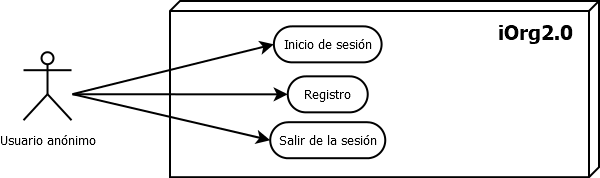
\includegraphics[width=1\textwidth]{../images/cu_anonimo.png}
  \caption{Diagrama de casos de uso actor usuario anónimo.}
  \label{fig:cu_anonimo}
  \end{center}
\end{figure}



\begin{figure}[!ht]
  \begin{center}
  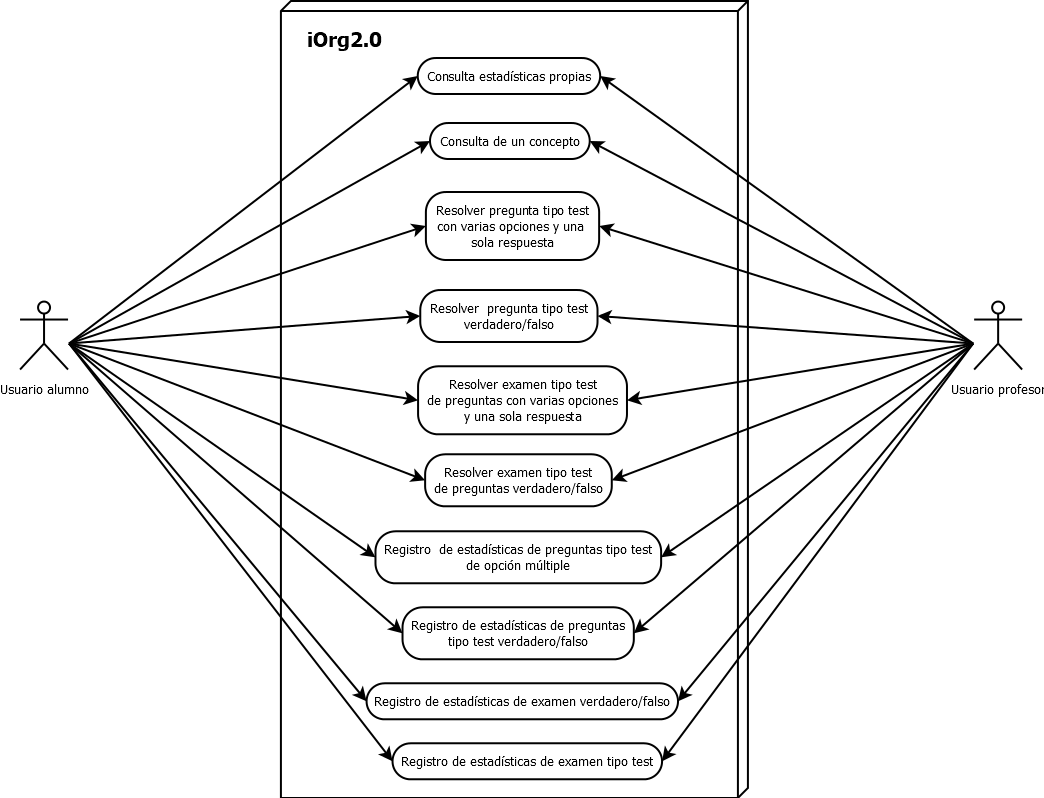
\includegraphics[width=1\textwidth]{../images/cu_alumno_profesor.png}
  \caption{Diagrama de casos de uso actores alumno y profesor.}
  \label{fig:cu_alumno_profesor}
  \end{center}
\end{figure}



\begin{figure}[!ht]
  \begin{center}
  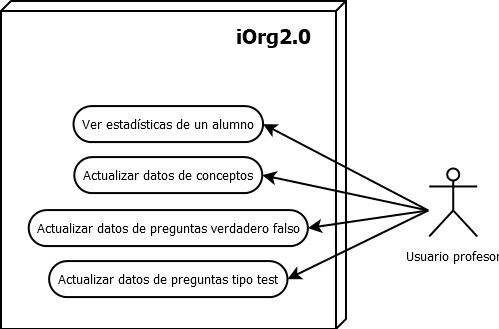
\includegraphics[width=1\textwidth]{../images/cu_profesor.png}
  \caption{Diagrama de casos de uso actor profesor.}
  \label{fig:cu_profesor}
  \end{center}
\end{figure}

\begin{figure}[!ht]
  \begin{center}
  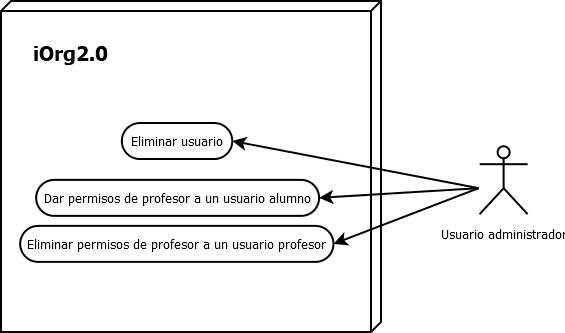
\includegraphics[width=1\textwidth]{../images/cu_administrador.png}
  \caption{Diagrama de casos de uso actor administrador.}
  \label{fig:cu_administrador}
  \end{center}
\end{figure}




\newpage

\section{Diagrama de navegación}

\bigskip
Aunque las secciones de esta aplicación no se preveen extensas en profundidad no está de más tener un diagrama donde mostrar la navegación:

\begin{figure}[!ht]
  \begin{center}
    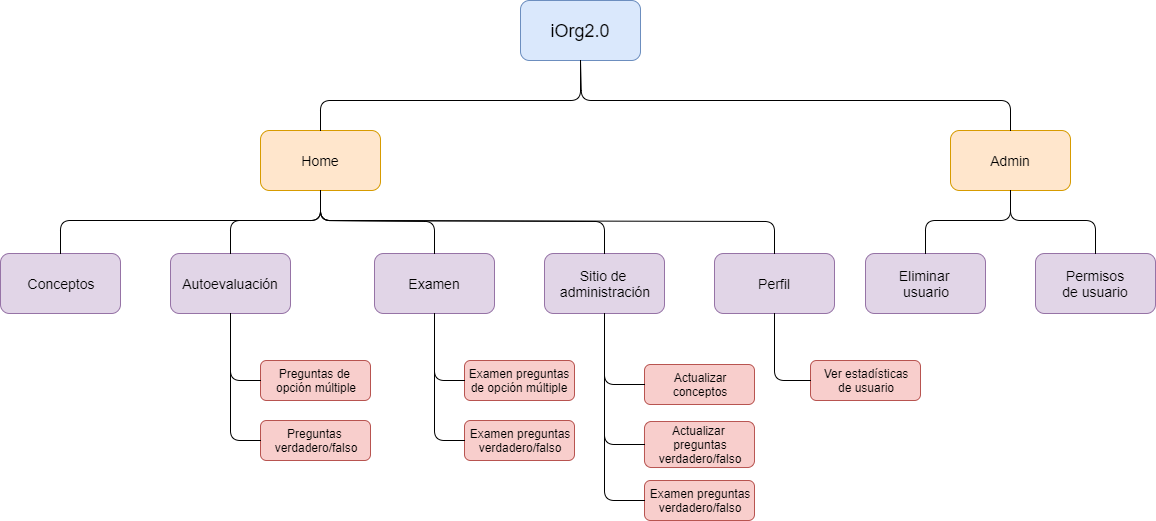
\includegraphics[width=1\textwidth]{../images/diagrama_navegacion.png}
    \caption{Diagrama de navegación}
    \label{fig:diagrama_navegacion}
  \end{center}
\end{figure}



%\chapter{Diseño e Implementación}


\section{Modelado de la base de datos}
En un primer diagrama para la base de datos se exponen las entidades y sus realciones. Atendiendo a los requisitos de la aplicación se plantea un diseño sencillo y directo en cuanto a las entidades y relaciones. En un primer esquema \textbf{entidad-relación} encontramos:



\begin{figure}[!ht]
  \begin{center}
    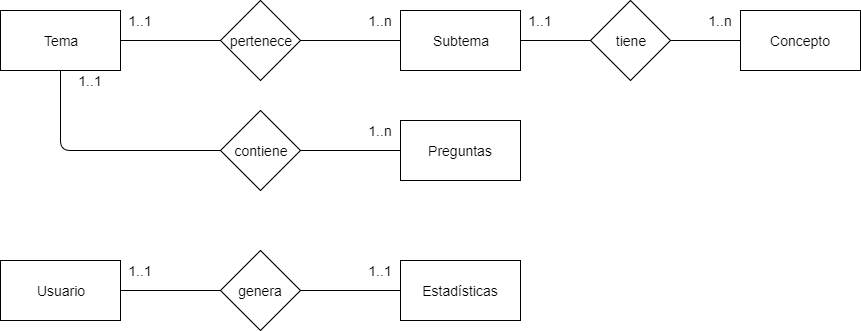
\includegraphics[width=1\textwidth]{../images/entidad_relacion.png}
    \caption{Entidad relación}
    \label{fig:entidad_relacion}
  \end{center}
\end{figure}


\bigskip
Analizando el diagrama vemos que las únicas relaciones que existen son de cardinalidad 1:N y 1:1.
Ambas las podemos simplificar eliminando la relación y añadiendo la clave primaria de la entidad con cardinalidad 1 en los campos de la entidad con cardinalidad N. Quedan así resumidas las tablas de la base de datos a únicamente las entidades:

\begin{figure}[!ht]
  \begin{center}
    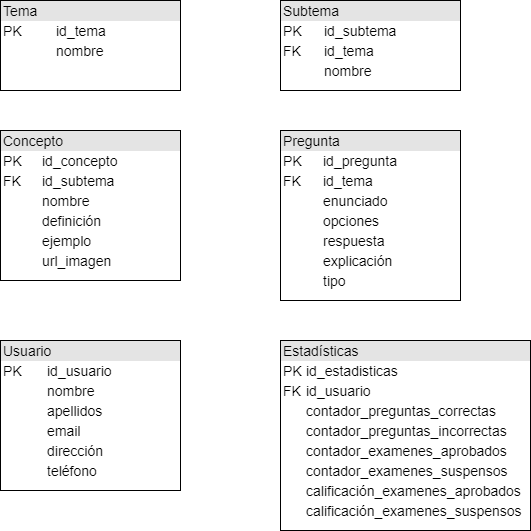
\includegraphics[width=1\textwidth]{../images/entidad_relacion_simplificado.png}
    \caption{Tablas del modelo entidad relación}
    \label{fig:entidad_relacion_simplificado}
  \end{center}
\end{figure}


\newpage

\section{Diseño de las interfaces}

A menudo y varias veces al día nos encontramos con cientos de interfaces\cite{user_exp2} con las que interactuamos, muchas de estas están tan asimiladas que ni las apreciamos. Las interfaces no son un objetivo para el usuario, si no que son el medio para llegar al él, siendo estas que no apreciamos las mejores interfaces. Una interfaz\cite{user_exp} no debe entorpecer el camino del usuario hasta su objetivo, debe ser sencilla, rápida de asimilar y directa.

\bigskip
Aquí mostramos algunos bocetos sencillos y su consiguiente implementación como interfaz de usuario en la aplicación:

\newpage

\subsection{Bocetos}

\begin{figure}[!ht]
  \begin{center}
    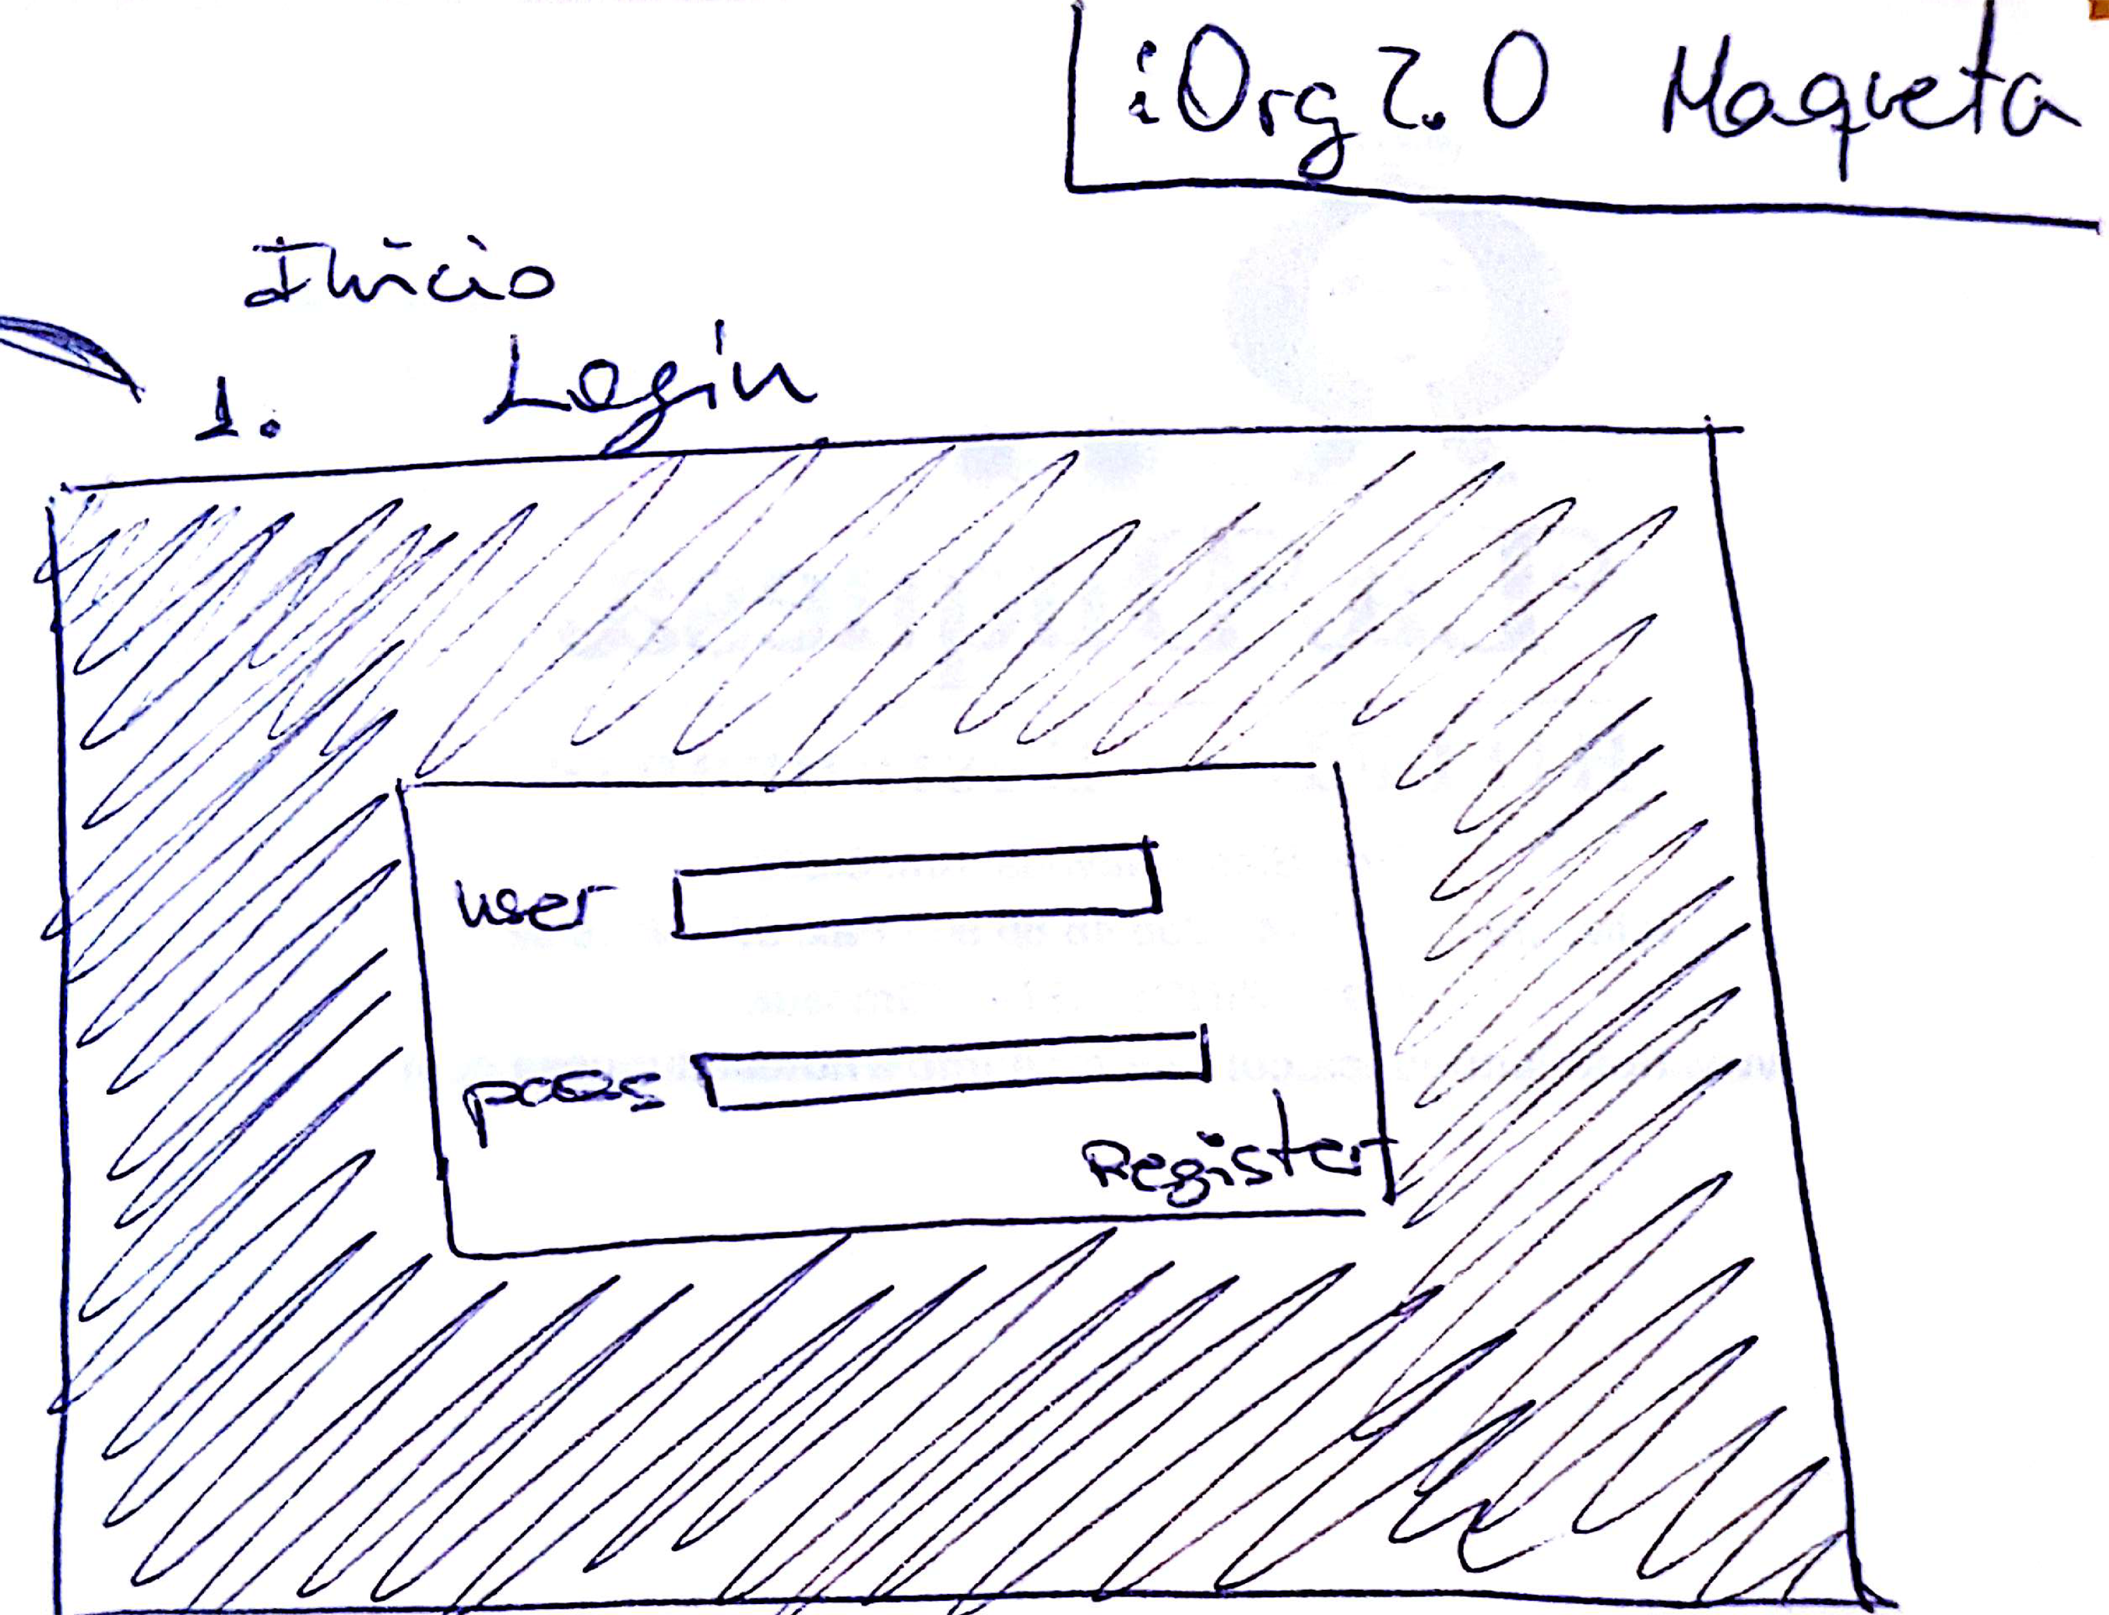
\includegraphics[width=1\textwidth]{../images/boceto_login.png}
    \caption{Boceto interfaz inicio de sesión.}
    \label{fig:boceto_login}
  \end{center}
\end{figure}


\begin{figure}[!ht]
  \begin{center}
    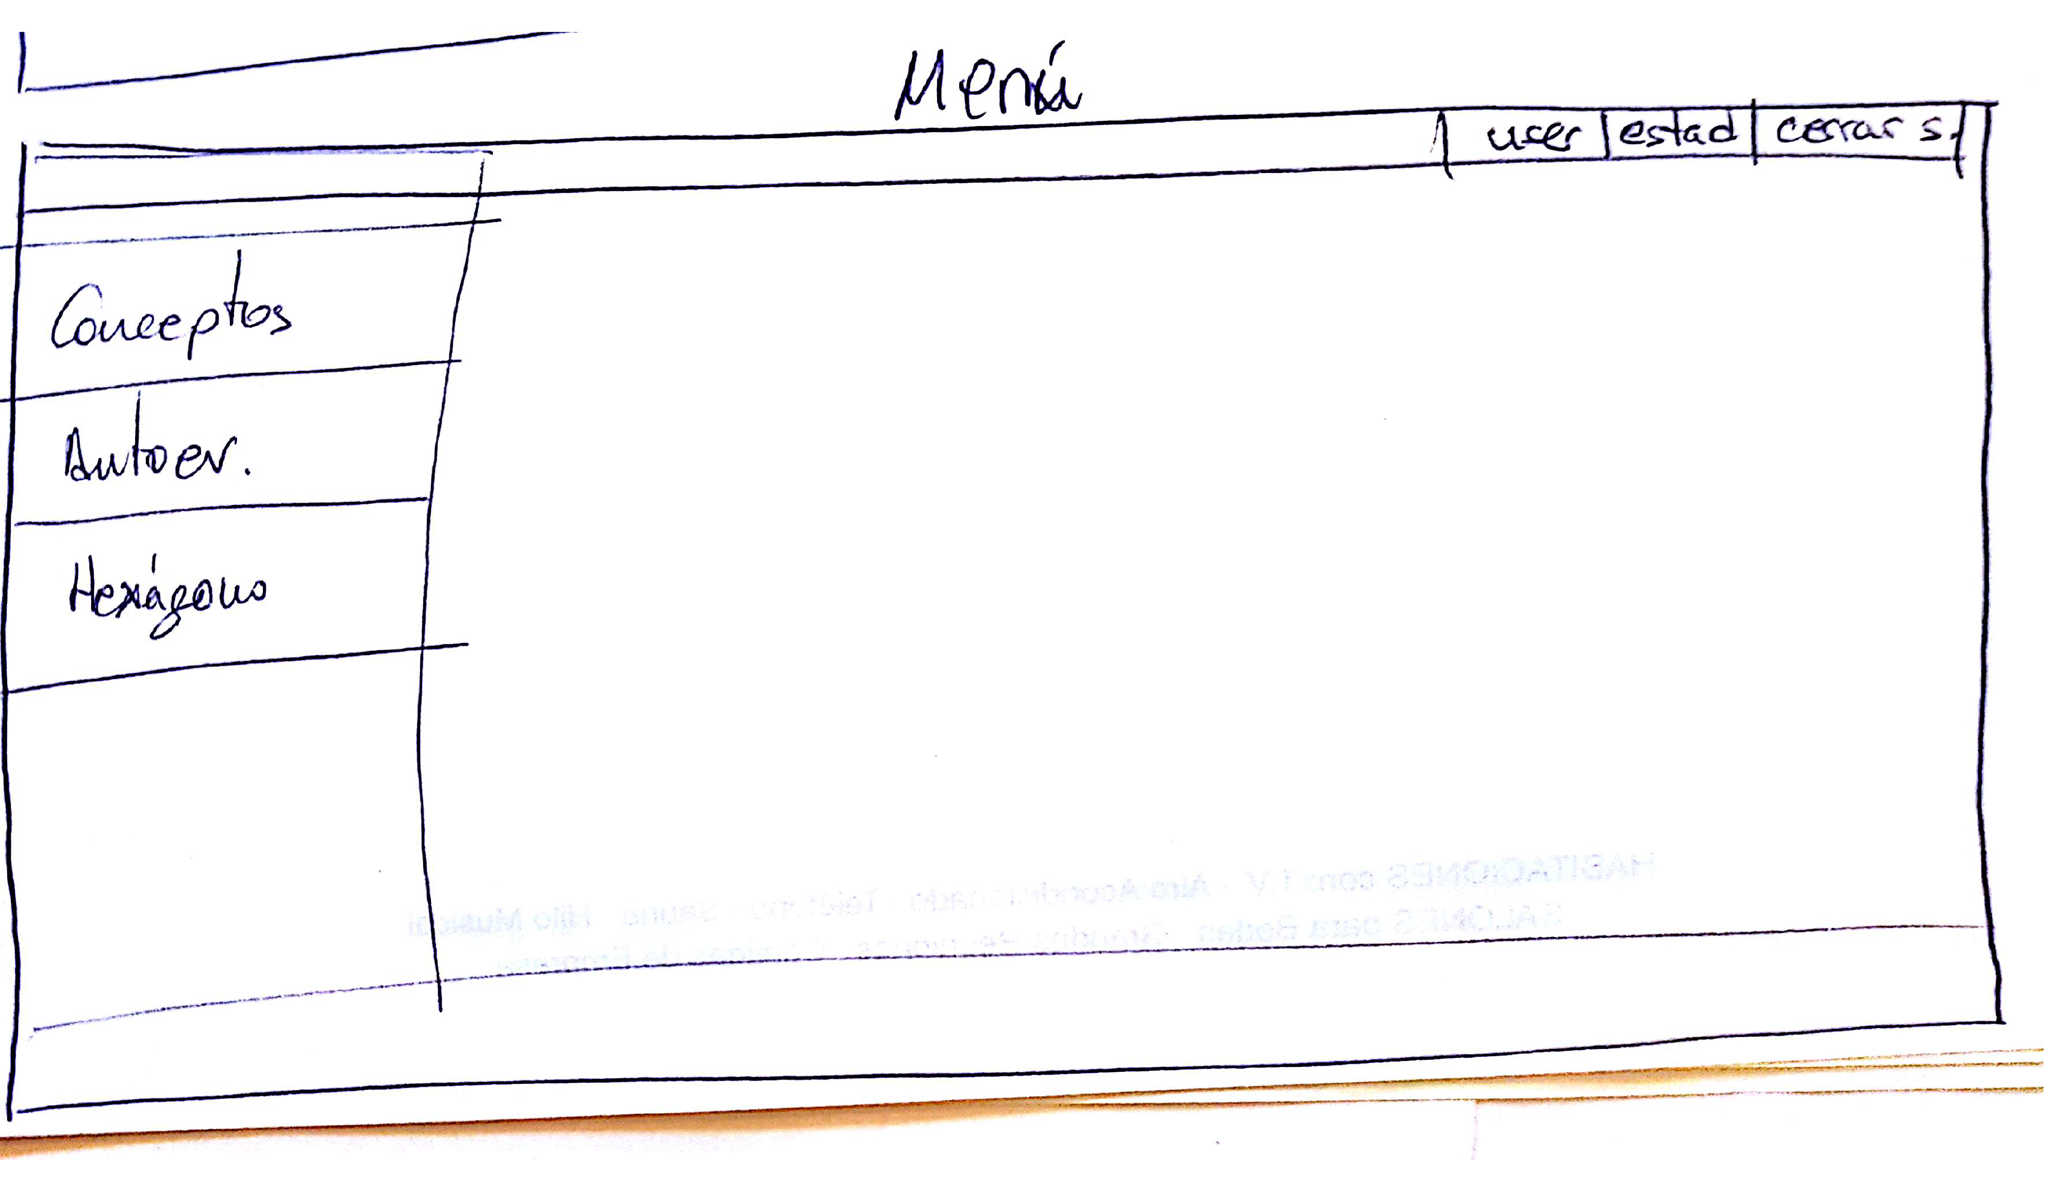
\includegraphics[width=1\textwidth]{../images/boceto_menu_lat.png}
    \caption{Boceto interfaz menú lateral.}
    \label{fig:boceto_menu_lat}
  \end{center}
\end{figure}



\begin{figure}[!ht]
  \begin{center}
    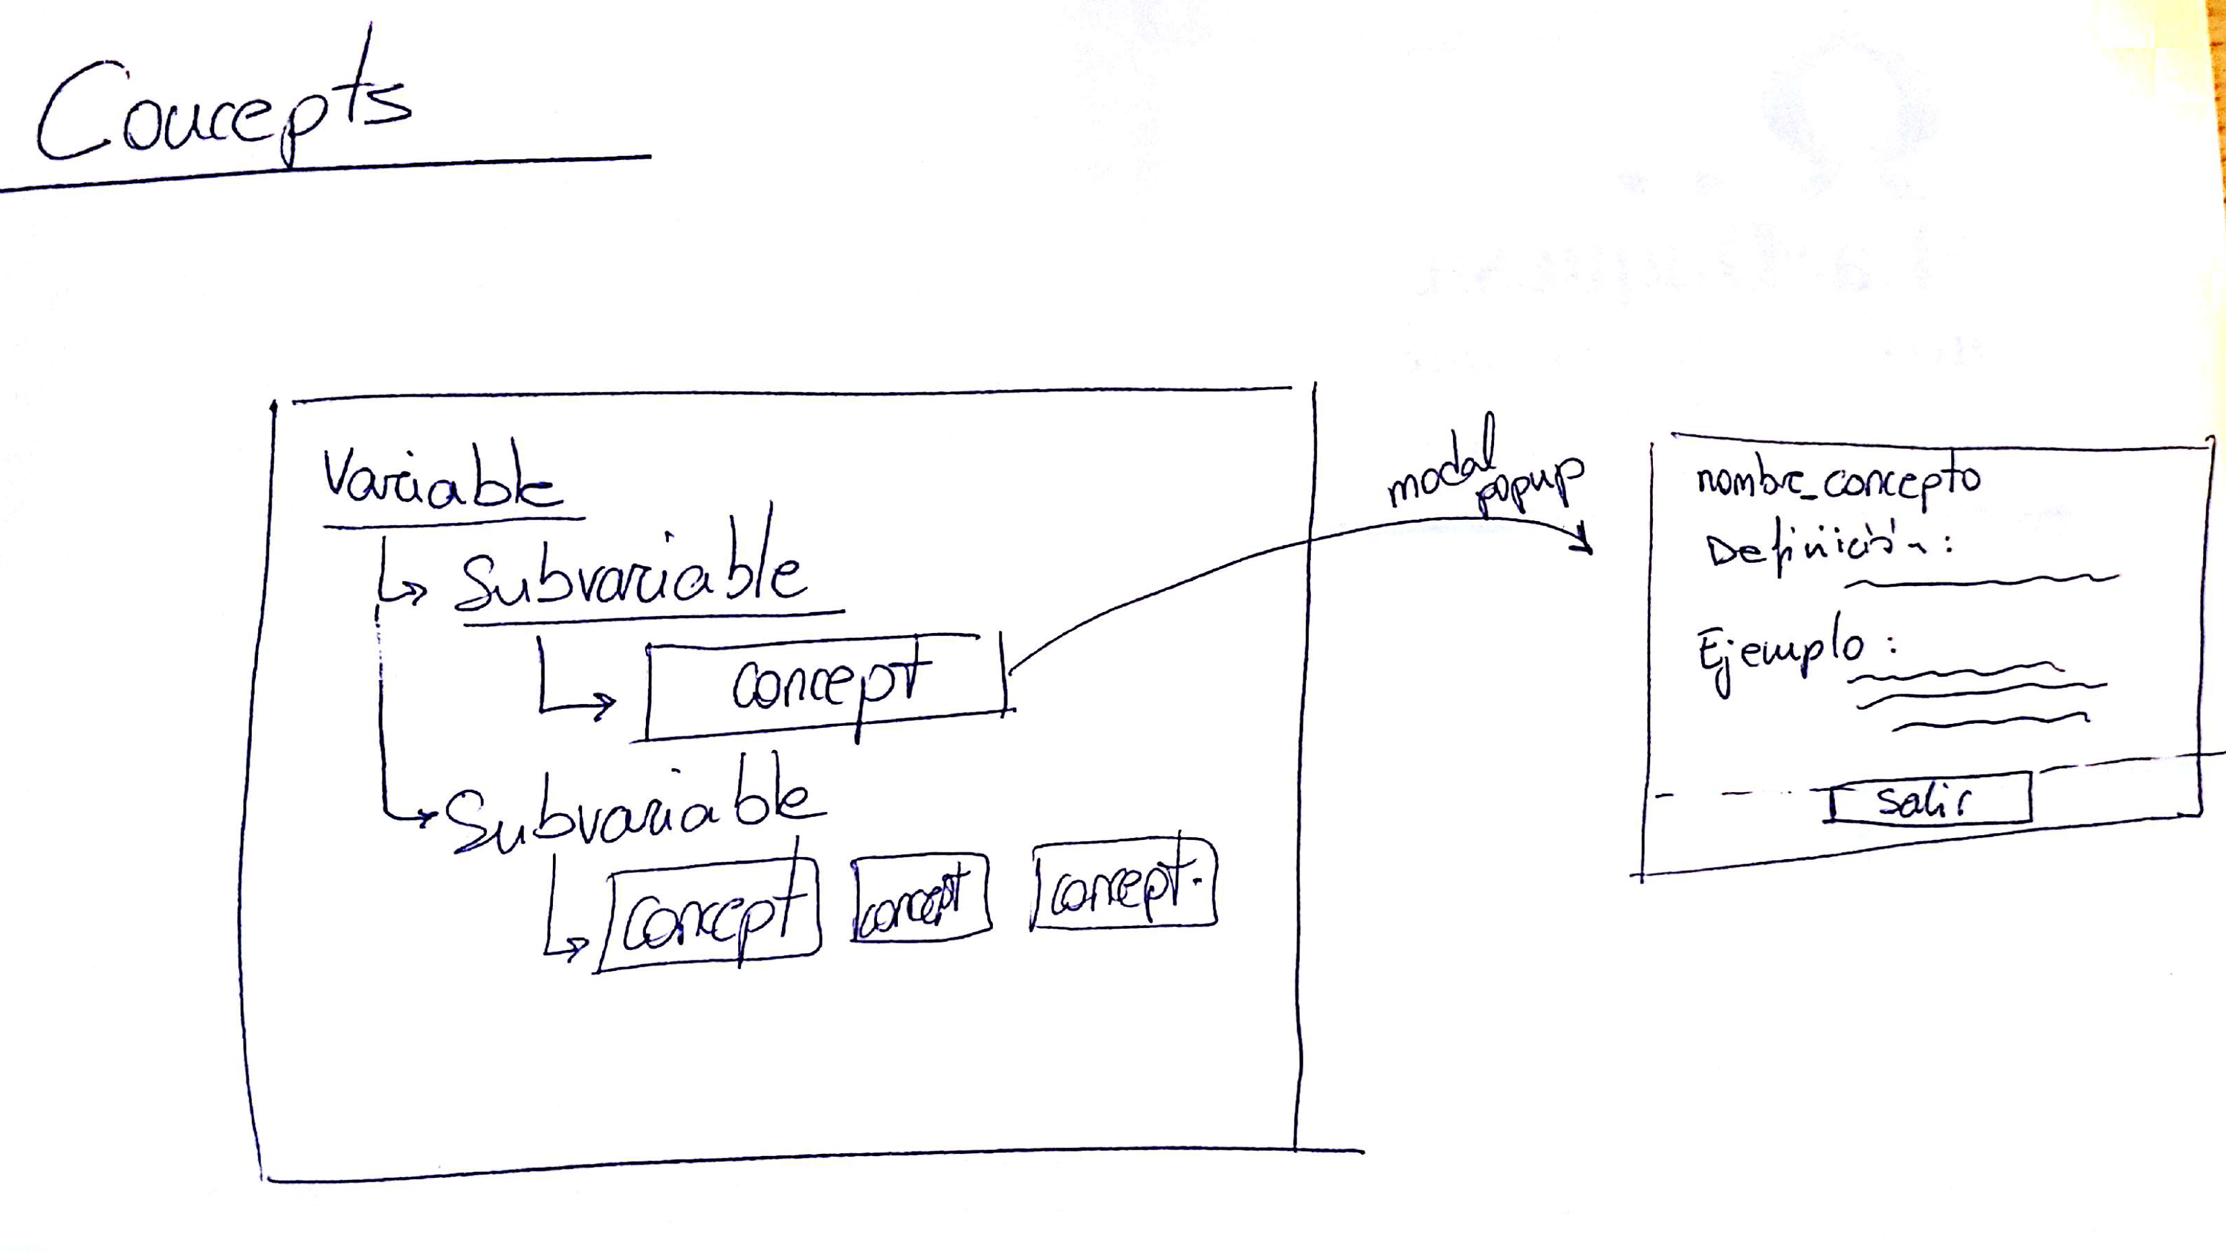
\includegraphics[width=1\textwidth]{../images/boceto_conceptos.png}
    \caption{Boceto interfaz conceptos.}
    \label{fig:boceto_conceptos}
  \end{center}
\end{figure}


\newpage

\subsection{Interfaz}

\begin{figure}[!ht]
  \begin{center}
    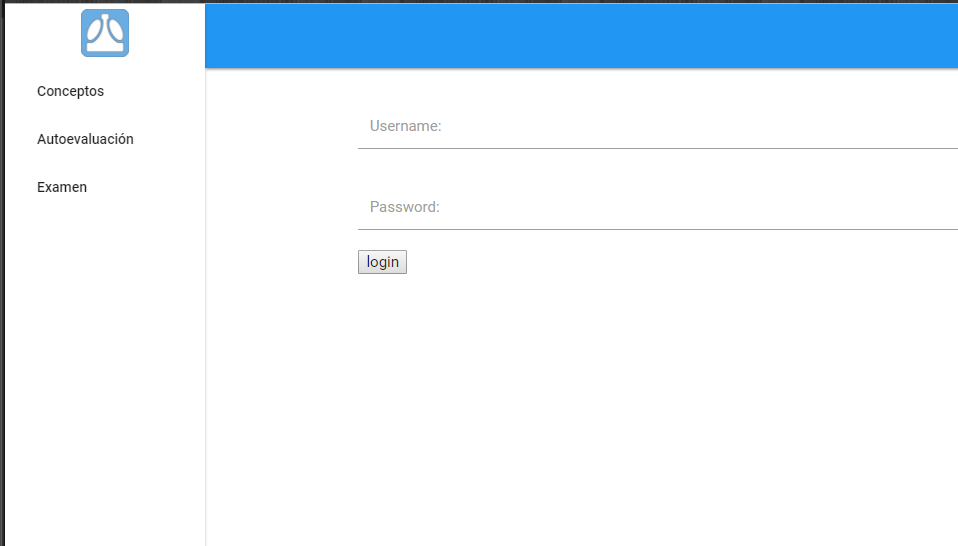
\includegraphics[width=1\textwidth]{../images/interfaz_login.png}
    \caption{Interfaz de usuario inicio de sesión.}
    \label{fig:interfaz_login}
  \end{center}
\end{figure}


\begin{figure}[!ht]
  \begin{center}
    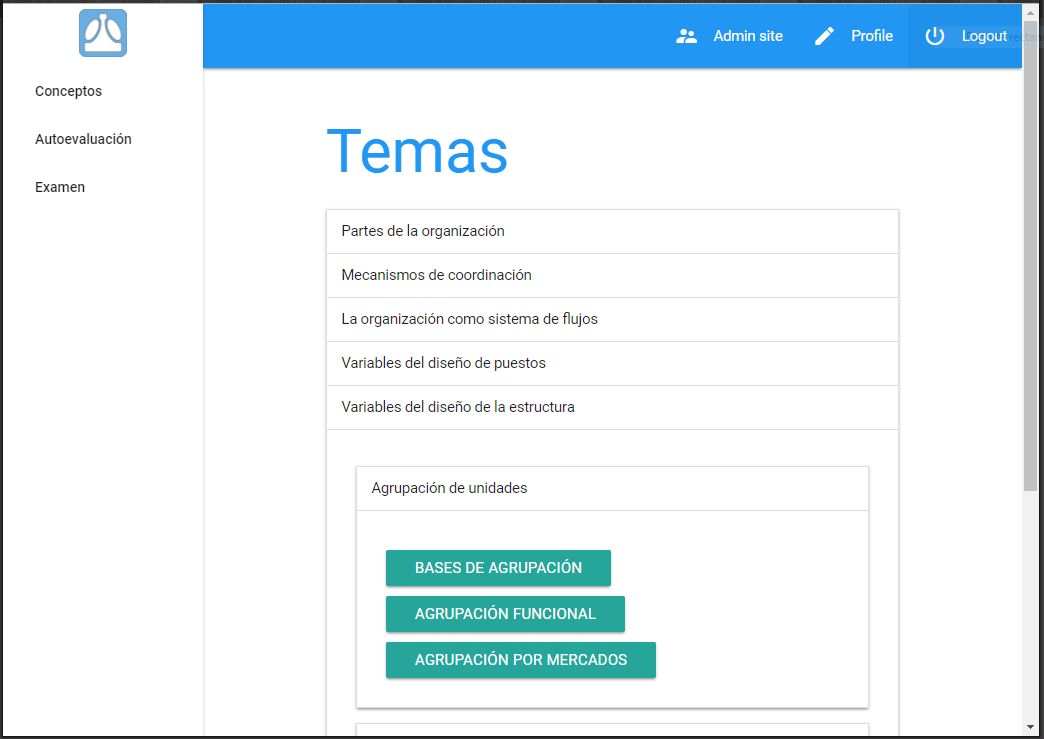
\includegraphics[width=1\textwidth]{../images/interfaz_conceptos1.png}
    \caption{Interfaz de usuario conceptos 1/2.}
    \label{fig:interfaz_conceptos1}
  \end{center}
\end{figure}



\begin{figure}[!ht]
  \begin{center}
    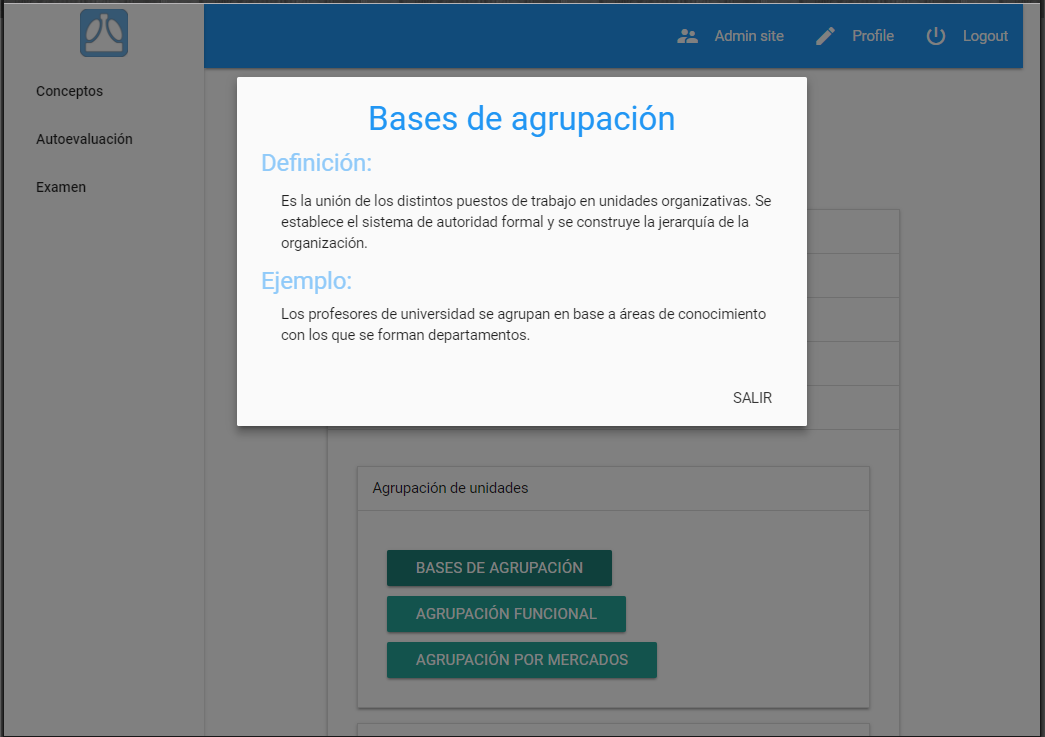
\includegraphics[width=1\textwidth]{../images/interfaz_conceptos2.png}
    \caption{Interfaz de usuario conceptos 2/2.}
    \label{fig:interfaz_conceptos2}
  \end{center}
\end{figure}


\begin{figure}[!ht]
  \begin{center}
    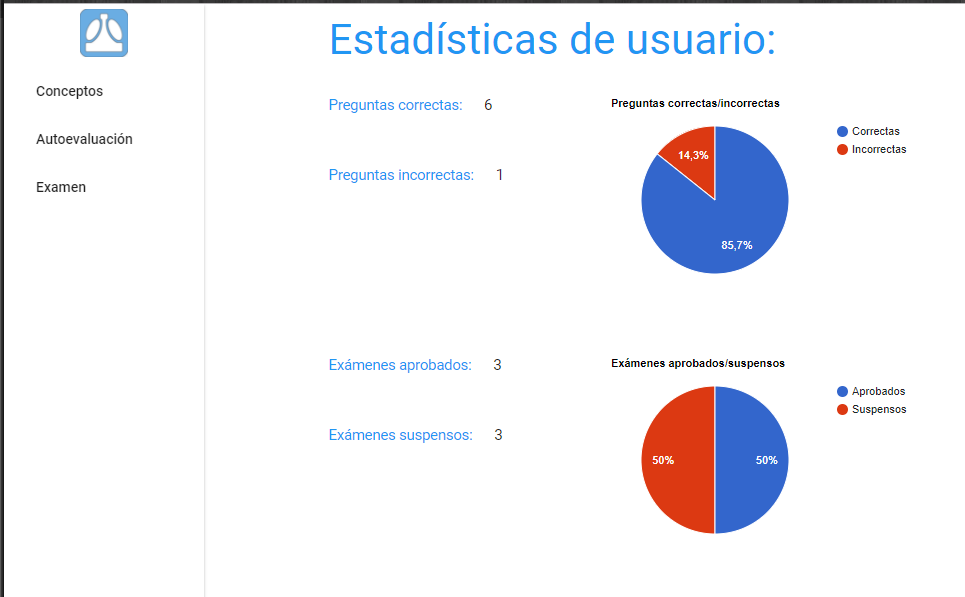
\includegraphics[width=1\textwidth]{../images/interfaz_estadisticas.png}
    \caption{Interfaz de usuario estadísticas de usuario.}
    \label{fig:interfaz_estadisticas}
  \end{center}
\end{figure}



\newpage

\section{Implementación}

Para una correcta y efectiva implementación destacaremos una vez más la importancia del proceso de análisis y diseño. Son en estas fases donde se asienta la implementación y si las anteriores se hicieron correcta y detalladamente esta fase se convierte en una mera interpretación o traducción de los análisis, diagramas y diseños anteriores. 

\bigskip
Para la fase de implementación es importante conocer las herramientas de las que podemos hacer uso. Nuestra aplicación se establece en un entorno web y ya hicimos un pequeño sondeo de las tecnologías que podíamos utilizar, ahora vamos a hablar brevemente de cómo hemos usado las herramientas y lenguajes en la implementación.

\bigskip
Vamos a distinguir entre lenguajes y herramientas usadas en el lado del cliente y lenguajes y herramientas usados en el lado del servidor:

\subsection{En el lado del servidor}
  En el lado del servidor tenemos Python como lenguaje y Django como framework.

\begin{itemize}
  \item \textbf{Django:} Framework web.
  \item \textbf{Python:} Lenguaje en el lado del servidor.
  \item \textbf{SQLite:} Sistema de gestión de base de datos.
\end{itemize}

\bigskip
Como ya explicamos unos capítulos atrás esta es nuestra elección para la parte del servidor. Una vez realizada la implementación podemos hablar de las experiencias con estas herramientas que ahora si, en mayor o menor medida, conocemos.

\bigskip
Lo primero que vamos a destacar es Django como framework web. Si bien es cierto que durante el {\grado} hemos trabajado con Django, lo hicimos dando unas ligeras pinceladas. En el desarrollo de este proyecto hemos podido comprobar la potencia de esta herramienta que abarca un amplio ámbito de componentes, desde la gestión de las rutas de nuestra aplicación pasando por la integración de los modelos y la base de datos hasta la gestión del controlador y las plantillas.

\bigskip
Con Django hemos conseguido abstraernos a un nivel un poco mayor de la gestión de la base de datos. Django trabaja con modelos, donde los desarrolladores definen sus ``entidades'' y Django se encarga de gestionarlas en la base de datos (que podemos definir en la configuración de Django) y en nuestro caso es SQLite\cite{sqlite}. Separar estos modelos nos permite, por ejemplo, cambiar la base de datos en cualquier momento y haciendo las migraciones necesarias, al hacer esto los modelos definidos en Django no sufrirán ninguna modificación.

\bigskip
De manera similar diferenciar entre los modelos, vistas y plantillas nos permite realizar un cambio en cualquiera de estos sistemas sin tener que cambiar sustancialmente el otro. Esto ha sido especialmente útil en este proyecto al cambiar la conexión de los modelos a las hojas de Google Drive. En una primera prueba de conexión entre Django y Google Drive, la lectura de varias celdas se hacía algo lenta. A medida que maduraba la implementación dimos con una forma de recorrer estos datos de manera más eficiente. La gestión de los modelos y el cambio que esto supuso no interfirió con las vistas ni las plantillas ya creadas lo que facilitó esta tarea.

\bigskip
También vamos a destacar que, a nuestro parecer, la curva de aprendizaje de Django es algo complicada. Se necesita tiempo para asimilar los diferentes conceptos que trabaja y los diferentes paquetes que podemos utilizar, cosa que creemos normal en un framework de estas dimensiones. A cambio, la potencia que ofrece este framework es más que notable.



\subsection{En el lado del cliente}

\begin{itemize}
  \item \textbf{Html5:} Lenguaje de marcado para las plantillas. 
  \item \textbf{CSS3:} Lenguaje que define los estilos de las plantillas.
  \item \textbf{LESS:} Precompilador CSS.
  \item \textbf{MaterializeCss:} Framework CSS ``responsive"\footnote{Que se adapta a varias resoluciones de pantalla}
  \item \textbf{jQuery:} Biblioteca multiplataforma de JavaScript.
\end{itemize}


\bigskip
Para mostrar la información en una aplicación web podríamos decir que lo básico que necesitamos es un lenguaje de marcado (Html5 \cite{html5}) y un lenguaje con el que definir sus estilos (CSS3 \cite{css3}). En nuestra aplicación, al igual que nos servimos de paquetes y frameworks en la parte del servidor para no rehacer funcionalidades a bajo nivel, en la parte del cliente nos basaremos en estilos ya predefinidos que nos ayudarán a dar un aspecto a la aplicación. Para esto hemos elegido MaterializeCss que nos permite agrupar los tamaños y colores de los elementos de la aplicación, así como facilitarnos funcionalidades como expandir y contraer listas, mostrar u ocultar el menú lateral en resoluciones de pantalla pequeñas, mostrar ventanas modales y crear la vista de formularios. Para esta interacción y la gestión de estos eventos se hace uso de jQuery.


\bigskip
Aunque relacionado con la parte del cliente no se especificaron muchos requisitos podemos hacer referencia al RNF-3 (\ref{rnf-3}) donde nos ha sido muy útil MaterializeCss ya que los elementos usados de este framework se ajustan a los diferentes tamaños de pantalla.



\subsection{Otras herramientas}

\begin{itemize}
  \item \textbf{PyCharm:} 
  \bigskip
    En general el uso de PyCharm como entorno de programación lo podemos calificar como positivo. Destacamos la ayuda que ofrece el entorno a la sintaxis del lenguaje, que al ser nuevo nos costó un poco al inicio de la implementación, o a la gestión y uso de las bibliotecas de Django por su extensión.
    \bigskip
    Señalar algunos puntos negativos que creemos que son comunes a cualquier entorno de programación y es la sensación de no saber qué está pasando en algunos momentos al incluir paquetes externos. Esto se produce por la automatización casi total de las funciones para agregar paquetes. Como caso particular al incluir el paquete de LESS el sistema no lo reconocía, tras varios intentos desinstalando e instalando con PyCharm se decidió hacerlo manualmente desde la terminal.

  \item \textbf{Git y Github:}
  \bigskip
   Ya describimos anteriormente Git pero creemos interesante contar las conclusiones sacadas de Git y Pycharm.
  
  \bigskip
  Ya en el {\grado} hemos hecho uso de Git como herramienta de control de versiones, pero siempre desde la terminal. La sincronización de Git y Pycharm resultó útil en cuanto a la visualización de ficheros incluidos en el repositorio y los que aún quedaban  por incluir o por subir al repositorio. Pycharm los cataloga con color verde (los actualizados en el repositorio), rojos(los que no están actualizados) y grises(los que no están incluidos). De esta forma en la barra lateral del entorno puedes ver rápidamente cómo están tus ficheros en el repositorio.
  
  \bigskip
  Por otro lado, la herramienta gráfica para la gestión del repositorio no resulta intuitiva y útil, quizá por ser usuarios asiduos a Git desde la terminal, pareciendo que no controlas completamente la actualización del repositorio. En este proyecto no se ha usado Git integrado con Pycharm y la gestión se ha realizado desde la terminal.
  
  \bigskip
  \textbf{GitHub} es una plataforma donde podemos conectar nuestros repositorios de Git de forma pública o privada. Los repositorios públicos forman una comunidad con código enorme de diferentes lenguajes y plataformas y con diferentes licencias de uso. 
  
  \bigskip
  En el proyecto hemos conectado Github con nuestros dos repositorios, uno se destina al código fuente y otro para el desarrollo en LaTex de esta misma documentación. El por qué de separar estos repositorios lo desarrollaremos más adelante.

  \begin{itemize}
    \item \textbf{Código fuente: }\href{https://github.com/rogegg/iOrg2}{https://github.com/rogegg/iOrg2} 
    \item \textbf{Documentación: }\href{https://github.com/rogegg/iOrg2_docu}{https://github.com/rogegg/iOrg2_docu} 
  \end{itemize}

  \item \textbf{Heroku:}
  \bigskip
  Heroku es una plataforma como servicio de computación en la Nube que soporta distintos lenguajes de programación. Esta plataforma nos va a permitir desplegar nuestro servidor en la nube y acercarnos al entorno final de producción de la aplicación. Llegados a este punto vemos interesante explicar cómo hemos hecho el despliegue y cómo hemos subido nuestra aplicación a la plataforma, vamos a extenderlo en el próximo capítulo.

\end{itemize}
%\input{chapters/07_Pruebas}
%\input{chapters/08_Difusion}
%\input{chapters/09_Conclusiones}
\appendix
%\input{chapters/user_manual}
%\input{chapters/devel_manual}

\backmatter

\newpage
\begin{thebibliography}{99}
	\addcontentsline{toc}{chapter}{Bibliografía}
\section{Bibliografía}


%autor, año de publicación, título y datos de la publicación (lugar y editorial).


\bibitem{python_blackbook}Byron Francis, 2016, ``Python : The Complete Beginners Guide (The Black Book)''. 
%Fecha de última consulta: 24/04/2017.


\bibitem{django_basic}Sergio Infante Montero, 2012, ``Curso Django. El framework para detallistas con deadlines'', Maestros del Web; Edición: 1.

\bibitem{ing_software}Ian Sommerville, 2011, ``Ingeniería de software'', Pearson Educación (9ª ed.) .





\section{Recursos Web}

\bibitem{python_wiki}``Web frameworks'', Wiki Python, Fecha de último acceso: 12/01/2017.\\\href{https://wiki.python.org/moin/WebFrameworks}{https://wiki.python.org/moin/WebFrameworks}

\bibitem{djangoproject}``Django'', Fecha de último acceso: 28/06/2017.\\\href{https://www.djangoproject.com/}{https://www.djangoproject.com/}

\bibitem{turbogears}``TurboGears'', Fecha de último acceso: 25/01/2017.\\\href{http://turbogears.org/}{http://turbogears.org/}


\bibitem{fullstackpython}``Books and tutorials for Django'', Full Stack Python, Fecha de último acceso: 12/02/2017.\\\href{https://www.fullstackpython.com/django.html}{https://www.fullstackpython.com/django.html}

\bibitem{modelo_desarrollo}``Implementación del modelo integral colaborativo'', José Luis Cendejas Valdéz, Fecha de último acceso: 21/02/2017.\\\href{http://www.eumed.net/tesis-doctorales/2014/jlcv/software.htm}{http://www.eumed.net/tesis-doctorales/2014/jlcv/software.htm}


\subsection{Otros recursos web}

\bibitem{shutter}``Herramienta de capturas de pantalla para Ubuntu'', Shutter, Fecha de último acceso: 15/02/2017.\\\href{http://shutter-project.org/}{http://shutter-project.org/}

\end{thebibliography}

\newpage \
\thispagestyle{empty}
\end{document}
